\documentclass[a4paper,11pt,french]{article}

\widowpenalty=9999
\clubpenalty=9999

\def\android{Android\texttrademark{}}

\usepackage[frenchb]{babel}
\usepackage[T1]{fontenc}
\usepackage[utf8]{inputenc}
\usepackage{um2/um2}
\usepackage{verbatim}
\usepackage{graphicx}


\setlength{\parindent}{0pt}
\setlength{\parskip}{2ex}


\title{Rapport de TER\\---\\Reconception du jeu Pticlic sous \android{}}
\author{Yoann \textsc{Bonavero} \and Bertrand \textsc{Brun} \and John \textsc{Charron} \and Georges \textsc{Dupéron}}

\begin{document}

\maketitle


\pagestyle{empty}
\thispagestyle{empty}

\tableofcontents


\pagestyle{empty}
\thispagestyle{empty}
\newpage
\setcounter{page}{1}
\pagestyle{plain}


\section{Introduction}

PtiClic\footnote{http://pticlic.org} est un jeu qui a été conçu et développé par Matthieu Lafourcade et Virginie Zampa. Le jeu a été créé afin de faire des études sur le vocabulaire et la sémantique sur des sujets de divers horizons dans un contexte ludique et motivant. Un mot central apparait, un nuage de mots entoure le mot central et le joueur clique et dépose des mots du nuage dans des catégories proposé sous forme d'énoncés. 

Par exemple, pour le mot central «bicyclette», les mots «pédale», «piéton», «pied», «automobile», «Sébastien Chabal», «Lance Armstrong», «pédalier», «voiture», «yeux», «rapide», «routier», «maillot», «pédaler», «dopage», «véhicule», «musclé», «nez», etc. sont proposés. Le joueur dépose ces mots dans les catégories «\dots{} est une partie de 'cycliste'», «Un contraire de 'cycliste' est \dots{}», «'cycliste' a un rapport avec \dots{}»,  «Une caractéristique de 'cycliste' est \dots{}» ou aucune de ces catégorie. Un score est obtenu en soustrayant les mots manquants et les mots incorrects aux mots corrects. 

Des linguistes et des informaticiens récupèrent les données liées aux parties jouées, ce qui leur permet de faire de la recherche dans leurs domaines respectifs.

Notre travail consiste à créer une version du PtiClic sous \android{}, une version modifiée du jeu adaptée pour téléphone mobile. Le sujet du TER définit clairement l'objectif de ce projet~:

\begin{quotation}
  L'étude et le prototypage d'une version fonctionnant sur \android{} semble intéressante. En particulier on s'intéressera à deux aspects :
  \begin{itemize}
  \item les contraintes imposées par l'environnement smartphone
  \item le biais qu'imposent ces contraintes sur le jeu et les données récoltées.
  \end{itemize}
  
  Il s'agira donc de modéliser une version adaptée aux smartphones et d'en implémenter un prototype fonctionnel.
\end{quotation}

Dans un premier temps, une version de base sera conçue et réalisée. Ensuite, des fonctionnalités supplémentaires seront ajoutées. La démarche adoptée par notre groupe est une approche itérative. Les quatres livraisons vont d'une version de base vers des versions plus élaborées~: un joueur pourrait, entre autres, modifier ses préférences ou choisir son niveau. L'idée est aussi de rendre le jeu plus attirant afin d'accroître le nombre de sujets participant aux études liées au résultat des données extraits des parties jouées.


\subsection{\android{}}

\android{} est un système d'exploitation pour téléphone mobile basé sur le noyau Linux développé par \android{} Inc., racheté par Google en 2005. Google et d'autres membres du Open Handset Alliance ont par la suite contribué à son développement et le \android{} Open Source Project (AOSP) est chargé de la maintenance et l'évolution d'\android{}. Ce système d'exploitation est utilisé notamment dans des smartphones, appelé aussi ordiphones, «terminaux de poche» ou «téléphones intelligents», produits et distribués par un grand nombre de fabriquants de téléphones mobiles. Le nombre de téléphones mobiles intégrant le système d'exploitation d'\android{} a cru sensiblement récemment.

Un grand nombre de développeurs ont créé des applications pour étendre la fonctionnalité des téléphones sous \android{} et il y a aujourd'hui
plus de 200 000 applications disponibles. Bien qu'\android{} Market soit le magasin en ligne opéré par Google, il existe d'autres distributeurs
d'applications \android{}. La majorité des applications sont écrites en Java, bien qu'il soit possible de développer des applications en
Python, en Ruby et d'autres par le biais du \android{} Scripting Environment.

 
\section{Analyse de l'existant}

L'application du jeu du PtiClic d'origine est une application disponible en ligne sur \url{http://www.lirmm.fr/pticlic/pticlic.php}. Nous
n'avions pas accès au code source de l'application ni à des diagrammes UML. La seule partie de cette application qui nous a été fournie est
une archive de la base de données dans un format textuel.

L'analyse de l'existant consistait donc d'une analyse du format et du contenu de cetta archive de la base de données ainsi que l'application sur Internet que nous avons testé et analysé.

\subsection{Le déroulement du jeu}
L'utilisateur clique sur le boutont «Je joue !». Un mot se dirige vers le centre de la page , c'est mot central. D'autres mots viennent entourer le mot central, ce sont les mots nuage. La police du mot central est plus grande que celle des mots nuages. Le mot central et les mots du nuage sont sont de couleurs contrastées.

\subsubsection{L'écran du jeu}
\begin{center}
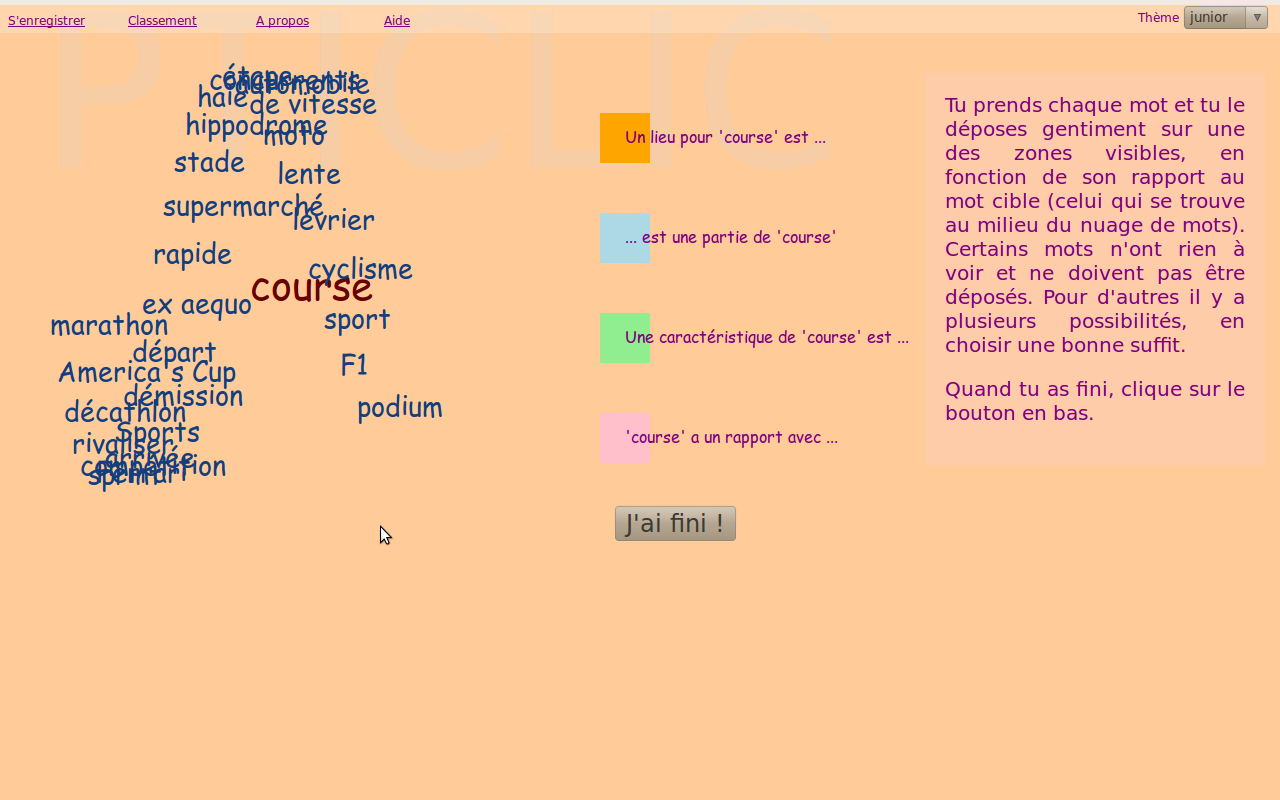
\includegraphics[width=14cm]{img/PtiClicJeu.png}
\end{center}

Les relations apparaissent à droite des mots. Une partie peut comporter de une à quatre relations. Un carré apparaît à droite de la relation suivi de la relation sous forme de syntagme tel que «\emph{(mot central)} est en rapport avec\dots{}», «Quoi/Qui pourrait \emph{(mot central)}~?». S'il y a plus d'une relation, les relations apparaîssent les unes en dessous les autres, toujours à droite des mots.

Encore plus à droite, un bref explicatif du principe du jeu, et tout en bas, le bouton «J'ai fini~!», 

Le principe du jeu est simple. Lorsque l'utilisateur estime qu'un mot nuage est lié au mot central par une des relations, il glisse et dépose le mot nuage sur le carré de la relation. Si l'utilisateur pense qu'aucune des relations ne convient, il laisse le mot dans le nuage tout simplement. 

\subsubsection{Déroulement de la partie}
\begin{center}
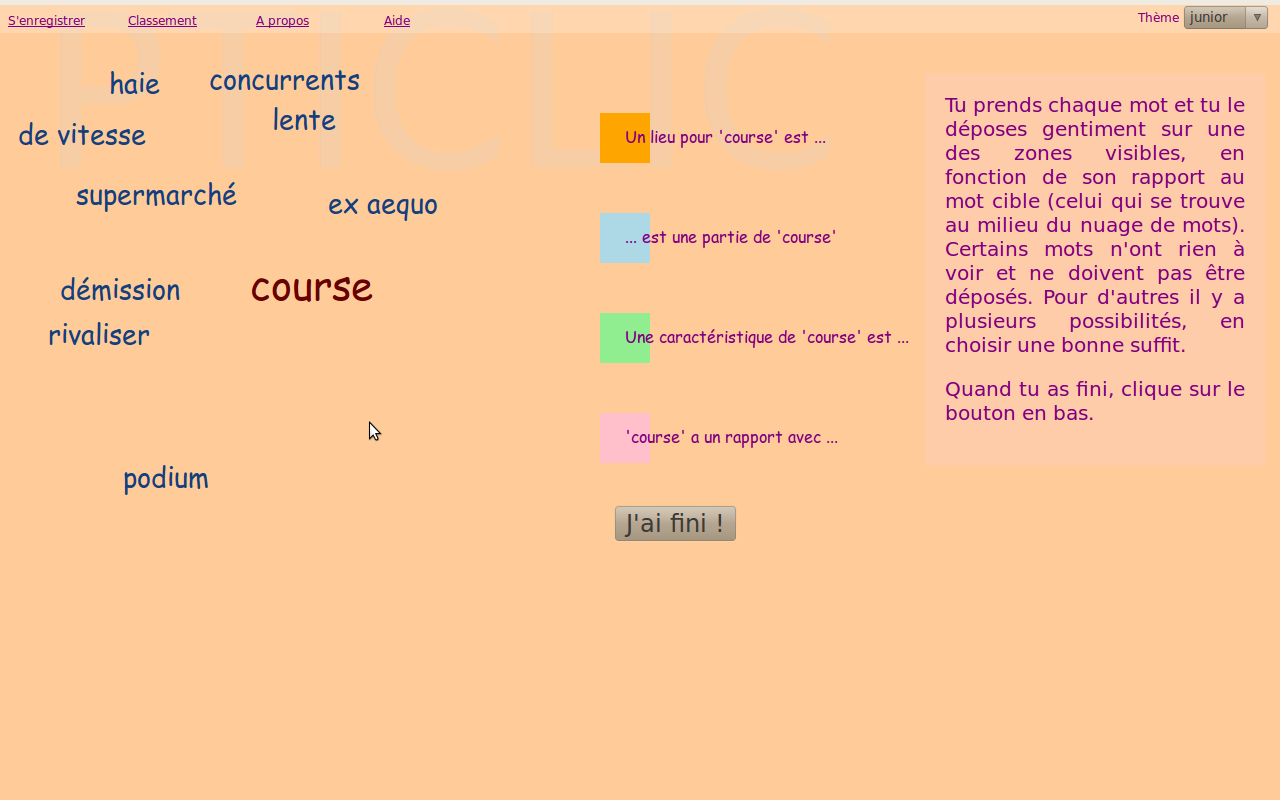
\includegraphics[width=14cm]{img/PtiClicJeu2.png}
\end{center}

Si le joueur se trompe, il peut double-cliquer sur le carré pour extraire le dernier mot déposé. En fait, le joueur peut double-cliquer
autant de fois qu'il le veut pour extraire tous les mots ayant été mis dans la relation un par en afin de modifier ses choix. Lorsque le
joueur a fait ses choix et souhaite finir sa partie, il clique sur «J'ai fini !», ce qui renvoie vers la page des résultats et du score. Il
n'y a aucune limite de temps pour terminer la partie.

\subsubsection{Score obtenu}
\begin{center}
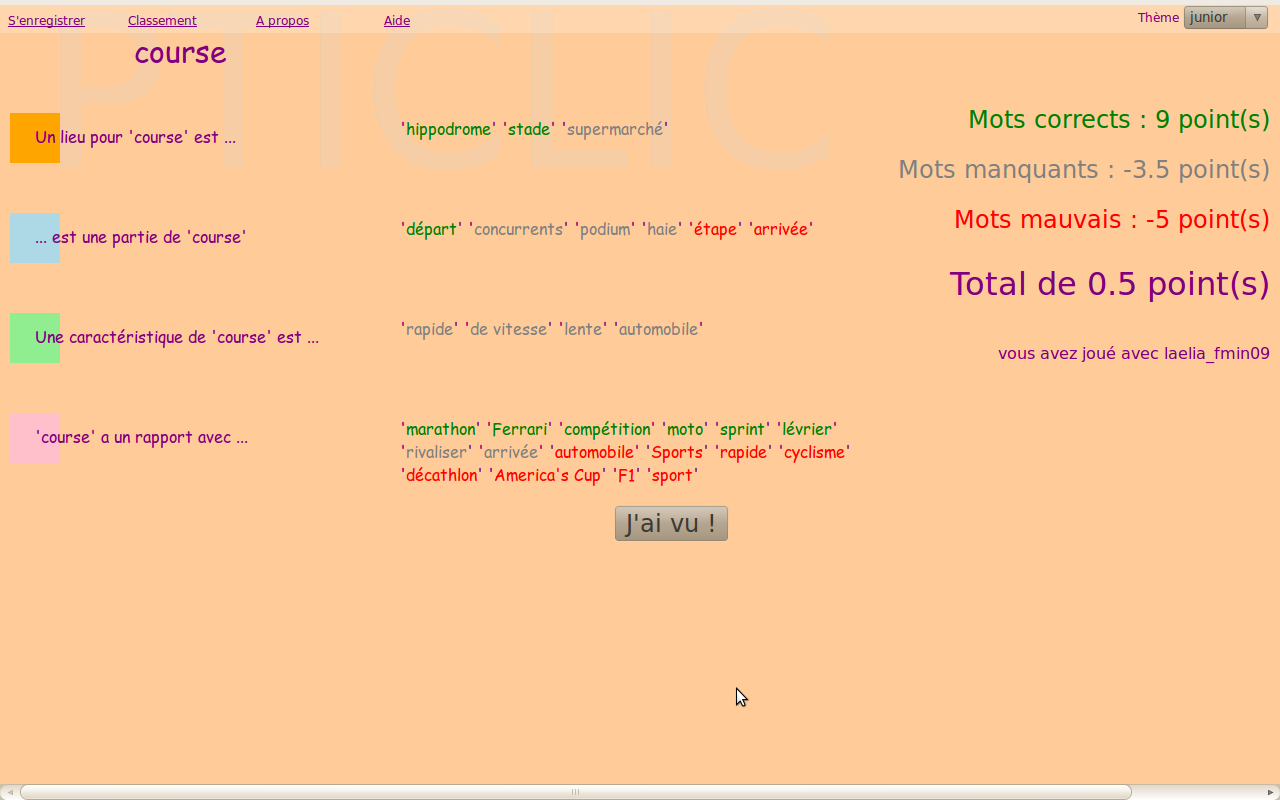
\includegraphics[width=14cm]{img/PtiClicResultats.png}
\end{center}

La page des scores contient aussi le corrigé de la partie. Les mots qui ont été mis dans la bonne categorie apparaissent en vert, les
mauvaises réponses en rouge et les omissions en gris. Un point est marqué par bonne réponse tandis qu'une mauvaise réponse ou une omission
fait perdre un demi-point. Lorsque deux réponses sont possibles, le point est marqué quelque soit la relation choisie. Le score final est
soit un entier, soit un entier plus un demi point~; il peut être négatif, nul ou positif.

Lorsque l'on clique sur le bouton «J'ai vu !», on retourne sur la page d'accueil.

\subsubsection{L'écran d'accueil du site}
\begin{center}
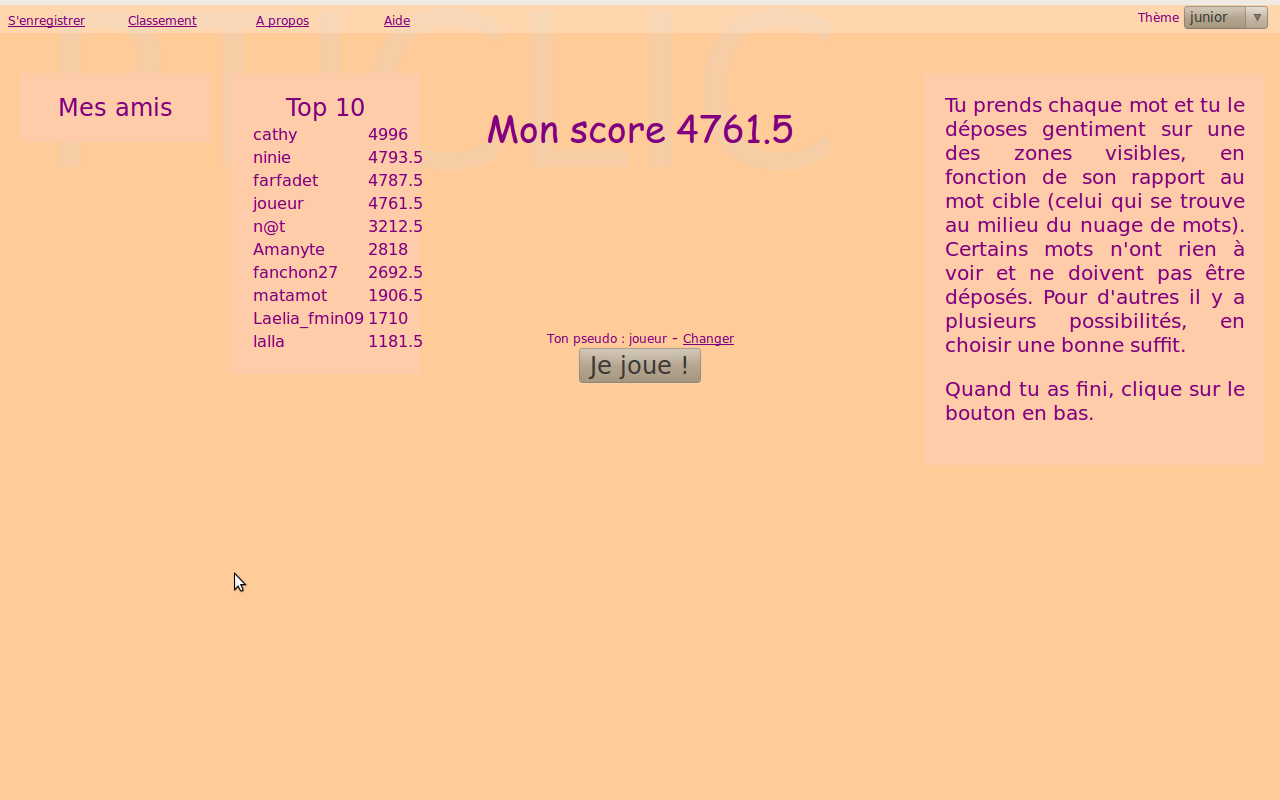
\includegraphics[width=14cm]{img/PtiClicAccueil.png}
\end{center}

Le joueur par défaut est l'utilisateur "joueur". Il est aussi possible de s'inscrire sur le site afin de créer son propre identifiant et mot
de passe afin de cumuler des points à chaque partie joué. Les dix joueurs qui ont cumulé le plus grand nombre de points sont inscrits sur la
liste des «Top 10». Les points cumulés par le joueur «joueur», qui est l'ensemble de parties jouées par des internautes non inscrits au
site, figure parmi les «Top 10». A droite de ceci, le score du joueur en question, c'est-à-dire, la somme totale des scores de toutes les
parties jouées par l'utilisateur. Si l'utilisateur veut jouer une partie de plus, il clique sur le bouton «Je joue !» en bas de la page et
une nouvelle partie est entamée.

Huit styles de couleurs sont disponibles et modifiables dans le menu déroulant en haut à droite de la page d'accueil. Lorsque le joueur s'authentifie avec succès, son identifiant apparaît dans le fond de page en très grande taille.

% TODO: MES AMIS ---> EXPLICATION DE COMMENT SONT CALCULES LES SCORES, C'EST PAR RAPPORT A UN AUTRE JOUEUR JE PENSE, ET NON PAS PAR RAPPORT A UN DICO... 

Lorsqu'un utilisateur souhaite s'inscrire au site, il est invité à lire un document explicatif de l'objectif du jeu dans le cadre du projet
de recherche de ce dernier. Il est aussi averti du contenu potentiel du jeu : comme les mots centraux et du nuage sont fournis par d'autres
utilisateurs, le vocabulaire rencontré peut ne pas convenir aux moins de 16 ans.



\subsection{Le dump de la base de données}

Le dump de la base de données est un fichier plat d'environ 2 000 000 lignes. Ce fichier contient un grand nombre de caractères accentués et
la version à notre disposition lorsque nous avons commencé à l'analyser, en extraire des données puis créer notre propre base de données,
n'était pas encodée en UTF-8 (bien qu'il y ait quelques mots qui soient encodés en UTF-8).

La base de données de laquelle est extraite ce dump provient d'un autre jeu de l'équipe TALN du Lirmm, nommé Jeuxdemots. Jeuxdemots propose
à l'utilisateur de donner des mots associés au mot central, ce qui, en quelque sorte, construit un nuage de mots. Cependant, les relations
entre le mot central et les mots du nuage ne peuvent pas être déterminées par Jeuxdemots, et c'est là le rôle de PtiClic.

Le dump contient en tout début des remerciements et quelques explications des acronymes et des abréviations utilisés, puis des statistiques, à savoir, le nombre d'occurrences de relations, la fréquence des noeuds, les 50 termes les plus fréquents. Plus un terme ou expression est fréquent, plus son poids est élevé. 

Le dump a proprement parler contient deux grandes parties~: une partie «noeuds» (\verb!NODES!) et une partie relations (\verb!RELATIONS!). La partie «noeuds»  contient non seulement des adjectifs, des adverbes, des substantifs et des verbes, mais aussi des locutions et des syntagmes, des mots tels que les prépositions, les conjonctions, les pronoms, les articles et les déterminants. Les substantifs peuvent être des noms propres, y compris des noms de lieux, des noms de personnes. 

Dans la partie "mots et expressions", chaque entrée -- chaque ligne -- contient un $eid$ (Entry IDentifier), un nom $n$ (name), un type $t$ et un poids $w$ (weight). En voici un exemple~:
\begin{verbatim}
eid=231064:n="pour femme":t=1:w=50
\end{verbatim}

Pour la partie relation, l'identifiant est le $rid$ (Relation IDentifier), le noeud de début $n1$ (starting node), le noeud de fin $n2$ (ending node), le $type$ (relation type) et le poids $w$ (weight). En voici un exemple~:
\begin{verbatim}
rid=430049:n1=82029:n2=151553:t=12:w=18
\end{verbatim}

\subsection{Analyse plus approfondie du jeu}
Bien que le dump de la base de données contienne 55 relations différentes, la version en ligne du jeu du PtiClic n'en utilise que treize (uniquement celles qui sont pertinentes pour le jeu)~:

\begin{itemize}

\item r\_associated|0|idée|Tout terme lié d'une façon ou d'une autre au mot cible\dots{} Ce mot vous fait penser à quoi~? \\
{\bf \verb![mot central]! est en rapport avec...} \\

\item r\_syn|5|synonyme|A partir d'un terme, il est demandé d'énumérer les synonymes ou quasi-synonymes de ce terme. \\
{\bf \verb![mot central]! a comme synonyme...} \\

\item r\_isa|6|générique|'animal' est un générique de «chat', «mammifère', «être vivant' etc. en sont d'autres\dots{} \\
{\bf \verb![mot central]! est une sorte de...}

\item r\_anto|7|contraire|'chaud' est le contraire de «froid', vous vous rappelez~? :) \\
{\bf Un contraire de \verb![mot central]! est...} \\

\item r\_hypo|8|spécifique|'mouche', «abeille', «guêpe' sont des spécifiques de «insecte»\dots{} \\
{\bf un spécifique de \verb![mot central]! est...} \\

\item r\_has\_part|9|partie|Il faut donner des parties/constituants/éléments du mot cible. Par exemple, «voiture» pourrait avoir comme parties : «porte», «roue», «moteur»\dots{} \\
{\bf ... est une partie de \verb![mot central]!} \\

\item r\_holo|10|tout|Le tout est ce qui contient l'objet en question. Pour «main', on aura «bras', «corps', «personne', etc. On peut aussi voir le tout comme l'ensemble auquel appartient un élément, comme «classe' pour «élève'. \\
{\bf \verb![mot central]! fait partie de...} \\

\item r\_agent|13|action>agent|L'agent (qu'on appelle aussi le sujet) est l'entité qui effectue l'action. Par exemple dans - Le chat mange la souris -, l'agent est le chat. Des agents typiques de «courir» peuvent être «sportif», «enfant»\dots{} \\
{\bf Quoi/Qui pourrait \verb![mot central]!~?} \\

\item r\_lieu|15|chose>lieu|A partir d'un nom d'objet (ou autre), il est demandé d'énumérer les lieux typiques où peut se trouver l'objet en question. \\
{\bf Un lieu pour \verb![mot central]! est...} \\

\item r\_instr|16|action>instrument|L'instrument est l'objet avec lequel on fait l'action. Dans - Il mange sa salade avec une fourchette -, fourchette est l'instrument. Des instruments typiques de «tuer» peuvent être «arme», «pistolet», «poison»\dots{} \\
{\bf Un instrument pour \verb![mot central]! est...} \\

\item r\_carac|17|caractéristique|Pour une terme donné, en général un objet, il est demandé d'énumérer les caractéristiques possibles et/ou typiques de cet objet. Par exemple, pour «eau' on pourra avoir «liquide', «froide', «chaude', etc. \\
{\bf Une caractéristique de \verb![mot central]! est...}

\item r\_lieu\_action|30|lieu>action|A partir d'un lieu, énumérer les action typiques possibles dans ce lieu.

\item r\_action\_lieu|31|action>lieu|A partir d'une action (un verbe), énumérer les lieux typiques possibles où peut être réalisée cette action.
{\bf Un lieu pour \verb![mot central]! est...} \\

\end{itemize}

D'autres relations qui figurent dans la base de données d'origine ne sont pas utilisées dans l'application~:

TODO: COMPLETER LES RELATIONS MANQUANTES, IL Y EN A 55 EN TOUT !

\begin{itemize}
\item r\_raff\_sem|1|raffinement sémantique|Raffinement sémantique vers un usage particulier du terme source

\item r\_raff\_morpho|2|raffinement morphologique|Raffinement morphologique vers un usage particulier du terme source

\item r\_domain|3|domaine|Il est demandé de fournir des domaines relatifs au mot cible. Par exemple, pour «corner', on pourra donner les domaines «football' ou «sport'.

\item r\_pos|4|r\_pos|Partie du discours (Nom, Verbe, Adjectif, Adverbe, etc.)

\item r\_holo|10|tout|Le tout est ce qui contient l'objet en question. Pour «main», on aura «bras», «corps», «personne', etc. On peut aussi voir le tout comme l'ensemble auquel appartient un élément, comme «classe' pour «élève'.

\item r\_locution|11|locution|A partir d'un terme, il est demandé d'énumérer les locutions, expression ou mots composés en rapport avec ce terme. Par exemple, pour «moulin', ou pourra avoir «moulin à vent', «moulin à eau', «moulin à café'. Pour «vendre', on pourra avoir «vendre la peau de l'ours avant de l'avoir tué', «vendre à perte', etc..

\item r\_flpot|12|potentiel de FL|(interne) potentiel de relation

\item r\_patient|14|action>patient|Le patient (qu'on appelle aussi l'objet) est l'entité qui subit l'action. Par exemple dans - Le chat mange la souris -, le patient est la souris. Des patients typiques de manger peuvent être «viande», «légume», «pain»\dots{}

\item r\_data|18|r\_data|Informations diverses

\item r\_lemma|19|r\_lemma|Le lemme

\item r\_magn|20|magn|La magnification ou amplification, par exemple - forte fièvre - ou - fièvre de cheval - pour fièvre. Ou encore - amour fou - pour amour, - peur bleue - pour peur.

\item r\_antimagn|21|antimagn|L'inverse de la magnification, par exemple - bruine - pour pluie.

\item r\_familly|22|famille|Des mots de la même famille sont demandés. Par exemple, pour «lait' on pourrait mettre «laitier', «laitage', «laiterie', etc.

\item r\_chunk\_pred|29|predicat|(interne) d'un chunk quel prédicat ?

\item r\_sentiment|32|sentiment|Pour un terme donné, évoquer des SENTIMENTS ou EMOTIONS que vous pourriez associer à ce terme. Par exemple, la joie, le plaisir, le dégoût, la peur, la haine, l'amour, l'indifférence, l'envie, etc.

\item r\_error|33|erreur|lien d'erreur

\item r\_maner|34|manière|De quelles MANIERES peut être effectuée l'action (le verbe) proposée. Il s'agira d'un adverbe ou d'un équivalent comme une locution adverbiale, par exemple : «rapidement', «sur le pouce», «goulûment», «salement»\dots{} pour «manger».

\item r\_meaning|35|sens/signification|Quels SENS/SIGNIFICATIONS pouvez vous donner au terme proposé. Il s'agira de termes évoquant chacun des sens possibles, par exemple : «forces de l'ordre», «contrat d'assurance», «police typographique»\dots{} pour «police».

\item r\_infopot|36|information potentielle|Information sémantique potentielle

\item r\_telic\_role|37|rôle télique|Le rôle télique indique le but ou la fonction du nom. Par exemple, couper pour couteau, scier pour scie, etc.

\item r\_agentif\_role|38|rôle agentif|Le rôle agentif indique le mode de création du nom. Par exemple, construire pour maison, rédiger ou imprimer pour livre, etc.

\item r\_causatif|42|cause|B (que vous devez donner) est une cause possible de A. A et B sont des verbes ou des noms.  Exemples : se blesser -> tomber ; vol -> pauvreté ; incendie -> négligence ; mort --> maladie ; etc.

\item r\_conseq|41|conséquence|B (que vous devez donner) est une conséquence possible de A. A et B sont des verbes ou des noms.  Exemples : tomber -> se blesser ; faim -> voler ; allumer -> incendie ; négligence --> accident ; etc.

\item r\_succession|52|succession|Qu'est ce qui peut SUIVRE (par exemple Noêl -> jour de l'an, guerre -> paix, jour -> nuit,  pluie -> beau temps, repas -> sieste, etc) le terme suivant :

\item r\_make|53|produit|Que peut PRODUIRE le terme ? (par exemple abeille -> miel)

\item r\_product\_of|54|est le produit de|Le terme est le RESULTAT/PRODUIT de quoi ?

\item r\_against|55|s'oppose à|A quoi le terme suivant S'OPPOSE/COMBAT/EMPECHE ?

\end{itemize}


Pour un mot central donné, seulement un nombre limité de relations sont possibles~:

TODO: INTEGRER L'ANALYSE PLUS APPROFONDIE ICI

SUBSTANTIF~: synonyme, contraire, spécifique, générique, partie, tout, lieu
VERB~: synonyme, contraire, lieu, instrument, agent
ADJECTIF~: synonyme, contraire
ADVERB~: synonyme, contraire

Les adverbes et LES locutions adverbiales sont relativement peu fréquents. La grande majorité des mots sont des substantifs, des verbes et des adjectifs ainsi que des locutions nominales, verbales et adjectivales. 

La relation "patient" est possible pour un mot central qui est un verbe, mais elle est plus complexe car elle ne fonctionnera que si le verbe en question est transitif. 

\section{Analyse des besoins}

\begin{quotation}
  L'étude et le prototypage d'une version fonctionnant sur \android{} semble intéressante. En particulier on s'intéressera à deux aspects :
  \begin{itemize}
  \item les contraintes imposées par l'environnement smartphone
  \item le biais qu'imposent ces contraintes sur le jeu et les données récoltées.
  \end{itemize}
  
  Il s'agira donc de modéliser une version adaptée aux smartphones et d'en implémenter un prototype fonctionnel.
\end{quotation}

\subsection{Les contraintes de l'environnement smartphone}

Comme tout outil, l'environnement smartphone présente à la fois des avantages et des inconvéniants. 

Les avantages sont nombreux~: un instrument portatif avec un bref temps de démarrage adapté à effectuer des tâches ponctuelles souvent de courte durée avec un écran tactile permettant d'agir directement sur des éléments affichés sur son écran. Le smartphone présente encore d'autres avantages, il est à la fois un lecteur mp3, un dictaphone, un appareil, un chronomètre et réveil, pour ne citer que quelques exemples.

Les inconvénients par rapport à un ordinateur classique sont aussi nombreux. L'écran est nettement plus petit limitant l'espace de travail
et obligeant davantage de navigation de page en page. L'entrée des données est plus difficile, il n'existe pas de clavier, ou bien seulement
un clavier virtuel ou un micro-clavier intégré. Malgré les avantages de l'écran tactile, son utilisation permet une précision bien moindre
que l'utilisation d'une souris à cause de la petite taille de l'écran et des doigts et mains qui bloquent la vue de l'écran lors du
glissement-et-déposé par exemple.

Le faible espace de stockage et les limites d'autonomie et d'énergie se traduisent par une nécessité d'économie de la part des concepteurs
d'applications par rapport aux ordinateurs classiques de plus en plus performants actuellement. C'est pour cette raison que le smartphone
n'est pas le plus adapté pour effectuer des tâches de longue haleine telles que l'édition de vidéos. Notamment, dans notre cas,
l'utilisation du réseau est lente, potentiellement coûteuse pour l'utilisateur (forfaits facturant à la quantité de données), et
consommatrice d'énergie.

Les applications bien adaptées au smartphone sont des applications telles que les calculatrices, les logiciels de prise de notes, les jeux
simples (casual games), et le jeu du PtiClic n'est pas une exception à cette dernière catégorie. L'avantage de ces applications sur un smartphone est
qu'il est possible d'y jouer lorsque l'on est en file d'attente à la Poste ou à la Préfecture ou bien dans les transports en commun. Un tel
prototypage du jeu demande toutefois une réflexion non seulement quant aux limites d'un smartphone mais aussi ses avantages.

Le jeu de base du PtiClic sous \android{} présente exactement les mêmes cas d'utilisations que l'application d'origine. 


\section{PtiClic et TALN}


Les projets JeuxDeMots et PtiClic s'inscrivent dans le domaine de la recherche en traitement automatique du langage naturel, et plus précisément dans celui du traitement de la sémantique du langage. Les données et les conclusions issues de ces projets pourraient contribuer directement ou indirectement à la recherche et à des applications en traduction automatique, l'indexation des textes, les correcteurs d'orthographes et de grammaires automatiques, la classification et la catégorisation des documents, des algorithmes de moteurs de recherche.


\subsection{Ferdiand de Saussure, la linguistique moderne, le TALN, JeuxDeMots et PtiClic}

Dans la partie qui suit, des notions de linguistique générale seront évoquées suivies d'une discussion d'applications dans le traitement automatique du langage naturel~: les dichotomies signifié-signifiant, l'arbitraire du signe, langue et parole, synchronie et diachronie. C'est Ferdinand de Saussure (1857-1913), fondateur de la linguistique moderne, qui a défini formellement pour la première fois ces concepts fondamentaux dans son Cours de linguistique général.\footnote{Ferdinand de Saussure, Cours de linguistique générale, édition originale~: 1916, édition 1979~: Payot, Paris. Il s'agit d'une oeuvre posthume rédigée à partir de notes de cours par deux disciples de Saussure~: Charles Bally et Albert Sechehaye. La publication de cet ouvrage marque le début de la linguistique moderne.}

\subsubsection{Le signe linguistique~: signifié, signifiant, référent}

Selon Saussure, le signe linguistique est une entité à deux faces~: le signifiant et le signifié. Ce principe semble assez simple. A un mot est associé un concept. Le mot 'cheval', c'est-à-dire son occurence orale ou écrite, le signifiant,\footnote{Pour Saussure, le signifiant est la version phonique d'un mot, ce qui est logique car la version graphique du mot n'est qu'une représentation écrite de la version phonique} nous évoque la représentation mentale que nous avons d'un cheval, le signifié. 


\begin{figure}[h!]
  \centering
      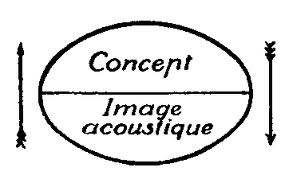
\includegraphics[width=0.5\textwidth]{img/signe-conceptimageacoustique.jpeg}
  \caption{Une représentation d'une idée, d'une chose, etc. est associée à la forme phonique d'un mot.}
\end{figure}

\begin{figure}[h!]
  \centering
      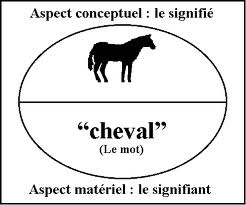
\includegraphics[width=0.5\textwidth]{img/signe-cheval.jpeg}
  \caption{A la représentation qu'on a d'un cheval est associé la forme phonique du mot cheval}
\end{figure}

Cette notion semble assez simple, mais, au contraire, la relation signifié-signifiant est très complexe. Cette entité a un très grand nombre de caractéristiques et le signifiant comprend des dénotations ainsi que des connotations qui peuvent être liées à des contextes multidimensionnels, généraux et spécifiques. Puis, à la notion de concept s'ajoute l'objet lui-même... s'il s'agit d'un objet physique~! Et s'il s'agit d'une émotion~? D'une action~? D'un sentiment~? D'une idée abstraite~? 

On peut aussi parler de sens figuré et de sens propre des mots. Par exemple au mot 'poésie' on pourrait associer les idées 'littérature', 'écrivain', 'auteur', 'strophes', etc. ... mais aussi 'musique', 'rêve', 'amour'. On parlera de ce deuxième sens lorsque l'on parle de la notion de 'bruit' dans la relation entre mots ou expressions. Et si on prennait en compte la polysémie d'un signifiant~?

Un demi-siècle plus tard, Emile Benveniste ajouta une autre dimension à ce schéma intégrant un 'référent' qui remplace le 'signifié', le 'signifié' étant, pour Benveniste, la dénotation du mot, c'est-à-dire bien l'objet lui-même. 

\begin{figure}[h!]
  \centering
      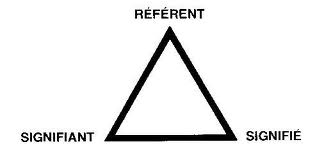
\includegraphics[width=0.5\textwidth]{img/trianglesemiotique.jpeg}
  \caption{Le signifiant de Saussure correspond au référent de Benveniste, le signifiant de Benveniste étant la dénotation du signifié alors que le référent est la représentation mentale ou 'concept' du signifié, qui englobe aussi des connotations qui peuvent être de nature très étendues telle que les contextes et les expériences personnelles que quelqu'un associe à un signifié.}
\end{figure}

Bien que ce modèle soit plus complet, cet ajout ne simple en rien notre travail. 

Un des obectifs des projets JeuxDeMots et PtiClic est d'établir des informations complexes concernant la représentation mentale d'un signifiant à travers ses liens avec d'autres signifiants. Bien que le langage soit limité, le langage demeure un des moyens de communication le plus efficace de l'homme.\footnote{'Un' des moyens les plus efficace car les images, les vidéos, etc. sont aussi des moyens de communication qui peuvent être aussi efficace que le langage. Cependant, dans la majorité des cas, le langage reste un mode de communication qui permet de s'exprimer avec le plus de précision} 

Dans le réseau lexical JeuxDeMots, le signifiant est élargi pour comprendre non seulement des mots mais aussi des locutions, des expressions et des raffinements sémantiques. Lorsqu'un mot est polysémique, il peut avoir plusieurs entrées distinctes. Par exemple, pour le mot 'boîte', on trouve 'boîte (contenant)', 'boîte (entreprise)', 'boîte (de nuit)', 'boîte (conserve)', etc.

On verra que dans le réseau lexical JeuxDeMots/PtiClic qu'il est possible de décrire à l'aide d'autres mots un grand nombre de traits sémantiques d'un signifiant à l'aide d'un nombre assez important de relations que ce signifiant entretient avec d'autres signifiants (relations sortantes). Qui plus est, les traits sémantiques du signifiant en question sont encore élargis car il est aussi possible d'associer à lui des signifiants dont il fournit des traits sémantiques (relations entrantes). 

\subsubsection{L'arbitraire du signe}

A l'exception de quelques onomatopés, le lien entre un mot (sous forme orale ou écrite) et son concept est complètement arbitraire. Le mot pour 'arbre' en anglais est 'tree', 'Baum' en allemand. Il n'y a aucun rapport entre la représentation phonique ou graphique d'un mot et sa signification.

Le fait que le signe linguistique est arbitraire rend le travail des chercheurs et des informaticiens en TALN bien plus difficile. Aucun élément dans le mot écrit (qui représente sa forme orale), ou plutôt d'une famille de mots, nous donne des indices quant au sens d'un mot. Il est toutefois possible de déduire le sens d'un mot à partir d'autres mots apparentés ou en se servant des notions d'étymologie provenant d'autres languages (par exemple, le latin et le grec) ou issues de la même langue. Cependant, cela peut aussi donner lieu à des faux amis ou des faux apparentés. 

Ce fait peut sembler évident, mais il est bien d'en être conscient. En effet, si le signe linguistique n'était pas arbitraire, il serait théoriquement possible d'écrire un algorithme pour déduire le sens d'un mot à partir du signifiant, c'est-à-dire le signifié à partir du signifiant, ce qui n'est pas le cas, d'où la complexité du problème que pose la sémantique. 


\subsubsection{Synchronie et diachronie}

La notion de synchronie correspond à l'étude ou l'analyse d'une langue à un moment donné, figé dans le temps. La diachronie, elle, s'intéresse à l'évolution d'une langue dans le temps.

Quoiqu'il soit intéressant d'étudier une langue à un moment donné dans le temps, cela ne correspond pas au monde réel. Une langue évolue quotidiennement grâce à ou à cause des nouveaux produits introduits sur le marché et les évènement politique et autre du monde entre autre. Il est donc important de pouvoir tenir compte de ces changements. La base de données de JeuxDeMots tient compte de ces changements grâce au fait que le réseau lexical évolue en temps réel ; le jeu qui alimente ce réseau est en ligne et est alimenté de manière continue. Une telle base de donnée permet aussi d'associer à de nouvelles entrées des dates précises. Il est aussi possible de se servir d'autres outils en TALN et en sémantique plus précisément pour mettre à jour une telle base de données, la LSA, l'analyse sémantique latente, par exemple, qui sera décrite ci-dessous.

Un exemple d'une application qui pourrait prendre en compte la diachronie est un moteur de recherche basé sur un réseau lexical qui est mis à jour en temps réel ou à intervalle de temps très court. Lors d'une histoire qui paraît à la une de tous les journaux concernant un homme politique ou un évènement catastrophique, les relations sémantiques qu'entretienne les mots maître de tels articles changent.

TODO:
-> article des inventeurs Lauder.... 
--> références...

\subsubsection{Langue et parole}

Une autre notion fondamentale de linguistique générale est la dichotomie 'langue' et 'parole'. La 'parole' est associée à l'acte individuel de langage alors que 'langue' est la représentation collective de l'ensemble des actes de parole dans l'esprit d'un locuteur natif. La 'parole' est hétérogène, individuel, active alors que 'langue' est collective, sociale, individuelle, passive. 

Enfin, pour avoir une représentation de signification qui est légitime, il est absolument nécessaire qu'il y ait un très grand nombre de sources et/ou de personnes qui alimentent le réseau lexical, sinon, les résultats risque d'être biaisés. Dans la dichotomie 'langue'/'parole' de Saussure, il est essentiel qu'un tel réseau soit une représentation sociale et homogène de la langue en question. Autrement dit, il faut que la base soit représentatif de la 'langue' et non pas de la 'parole' ni quelque part entre 'langue' et 'parole'. Ceci implique qu'il faut aussi des données d'une diversité de sources et de types de sources~: sources écrites et orales, de plusieurs domaines, de plusieurs niveaux de langue. 

D'emblée, la base de données JeuxDeMots/PtiClic n'est pas 'parole' pure car il est nécessaire que deux utilisateurs donne les mêmes réponses, que ce soit concernant le lexique ou les relations sémantiques, sinon, la réponse d'un seul utilisateur n'est pas validée. En outre, le fait que le poids d'une relation augmente lorsque plusieurs paires d'utilisateurs donnent la même réponse tend vers la 'langue' plutôt que vers la 'parole'. Enfin, il est souhaitable qu'un très grand nombre d'utilisateurs contribuent à la base de données JeuxDeMots parce que, justement, il faut que les informations contenues dans la base relève de réellement de 'langue' selon le sens saussurien de ce mot. 

TODO: 
myriadisation du travail (beaucoup de gens qui travaille)
 / parcellisation (couper les taches en petites taches)
lexico-sémantique
redondance~: poids, chauvauchement... pour renforcer, etc.
 



\subsection{Le réseau lexical JeuxDeMots}

La base de données utilisée pour PtiClic est la même de celle utilisée pour JeuxDeMots, ou, dit de manière plus précise, PtiClic utilise la base de données de JeuxDeMots. Les nouveaux termes, ou noeuds, sont introduit dans le jeu JeuxDeMots ainsi que de nouvelles relations, mais l'objectif principal de PtiClic est d'introduire de nouvelles relations parmi des noeuds existants. Il n'est pas possible d'ajouter de nouveaux noeuds lors d'une partie de PtiClic, seulement de nouvelles relations. 

Un noeud peut correspondre à un mot ("pomme"), une expression ("avant toute chose"), c'est le noeud de type 1. Ces termes figureront dans le mot central et les mots nuage de nos parties. Le noeud de type 4 sont ceux associés avec la catégorie grammaticale des mots et contient les attributs genre et nombre également ("Adj:Fem+SG:InvGen+PL"). D'autres métadonnées concernant les noeuds de type un se trouve dans les noeuds de type 18 qui nous donnent des informations concernant le niveau de langue ("Langue:soutenu", "Langue:familier") et la transitivité des verbes ("Ver:Intransitif") entre autre. 

Les noeuds de type 36 nous donnes des informations très utiles concernant la nature des mots bien plus précis que la catégorie grammaticale. Par exemple, si nous souhaitons que les réponses possibles soit non seulement un nom mais aussi une chose, on pourrait filtrer les résultats grâce au noeud "\_INFO-SEM-THING". Si l'on souhaite que les réponses possibles soit des évènements, des personnes ou des lieux, on peut se servir des relations "\_INFO-SEM-EVENT", "\_INFO-SEM-PERS" et "\_INFO-SEM-PLACE" respectivement, encore faut-il / pourvu ... que des relations vers ces noeuds soit alimentées préalablement. 

Cinquante-cinq différentes types de relations existent qui donneraient des informations de nature morphologique, syntaxique, sémantique, pragmatique et métalinguistique. 

Il existe environ 230 000 noeuds de type 1 (term). Moins de 106 000 de ces mots contiennent des relations sortantes de type 0 (idée), qui est le type de relation le plus général dont presque toutes les autres relations sémantiques sont des sous-ensembles, ce qui représente moins de 50\% des noeuds. Si on prend l'ensemble des relations existant dans la version originale du jeu PtiClic, seulement 122 000 noeuds ont des relations sortantes et moins d'un quart des noeuds du réseau lexical ont des relations entrantes. 

Il serait intéressant d'introduire de nouvelles relations entrantes et sortantes là où il en existe aucune. Toutefois, il serait très difficile voire impossible à partir des relations déjà existantes. Si l'on introduit des mots par hasard dans le nuage, il serait très improbable qu'il y ait des relations avec un mot central, aussi choisi par hasard. Les joueurs du PtiClic ne s'intéresseraient plus au jeu et l'alimentation de la base sera ralentie voir stoppée. Il faudrait un moyen auxiliaire pour introduire de nouvelles relations de ce genre dans la base.  

\subsection{LSA et le réseau lexical JeuxDeMots}

PtiClic combine deux moyens pour la création d'une partie, c'est-à-dire les combinaisons mot central et mots nuages~: LSA et le réseau lexical JeuxDeMots.\footnote{Il semblerait que PtiClic a à un moment donné utilisé ces deux modes afin d'établir des relations sémantiques entre tous les noeuds~: "PtiClic [...] se fondent sur deux méthodes d’acquisition lexicale et ontologique~: l'Analyse Sémantique Latente (LSA) et JeuxDeMots (JDM). (Il est intéressant) de combiner ces deux méthodes afin de combler les lacunes de chacune au travers de (ce) jeux. (...) [C]e jeu permet une double acquisition~: acquisition de vocabulaire par les utilisateurs et acquisition lexicale par la machine. Ceci a donc un intérêt à la fois en TICE et en TALN. Avant de parler de la génération de parties, une explication des deux approches s'impose. Une brève description de ces deux moyens d'analyse sémantique sera donnée dans cette partie." ... "Nous partons d’un réseau déjà existant, celui de JeuxDeMots (http://jeuxdemots.org) et de LSA (latent semantic analysis) qui permet, à partir de textes, de trouver des termes proches d’un terme donné (dans le même champ lexical)." ... "Nous constatons que pour un terme donné, les mots proches fournis par LSA sont couvrent l'ensemble des relations issues de JDM mais que les relations pertinentes restent à identifier." (PtiClic et PtiClic-kids~: Jeux avec les mots permettant une double acquisition. In proc TICE 2010, 7e coloque TICE, Nancy~: 6-8 décembre 2010) (TICE = Technologie de l'Information et de la Communication pour l'Enseignement). Toutefois, selon une discussion avec Mathieu Lafourcade le 4 mai 2011, cela n'est plus le cas et la LSA ne serait pas très efficace lorsqu'elle est appliquée dans la création de partie de PtiClic. Toutefois, étant donné que la moitié des noeuds n'ont aucune relation sémantique entrantes ni sortantes, il est nécessaire d'utiliser d'autres moyens que les relations existantes dans le seul réseau lexical JeuxDeMots afin de créer de nouvelles relations mettant en jeu ces mots. Bien que ceci dépasse le sujet de ce TER, on évoquera ce problème de cette lacune et la LSA dans la suite de la présente discussion.}


\subsubsection{La LSA}

Il existe plusieurs systèmes et algorithmes pour évaluer le rapport sémantique entre des mots. Une méthode consiste à chiffrer le lien entre deux mots. Si l'on représente ces liens par un graphe, il y aurait un seul lien ou arc entre deux mots ou noeuds donnés et une valeur associée à la relation qu'entretiennent ces deux mots. Un tel système est la LSA\footnote{'LSA' signifie en anglais Latent Semantic Analysis, ce qui se traduit en français 'Analyse sémantique latente'}. 

Sans rentrer dans les détails de l'algorithme de la LSA, qui est brevetée et payante, cette approche consiste à générer un graphe de relations entre mots à partir de textes écrits. Le résultat de l'algorithme donne un graphe de noeuds (mots) et d'arcs (estimation du degré de lien sémantique entre deux mots) comme suit~:


\begin{figure}
 \begin{minipage}{\textwidth}
\centering 
       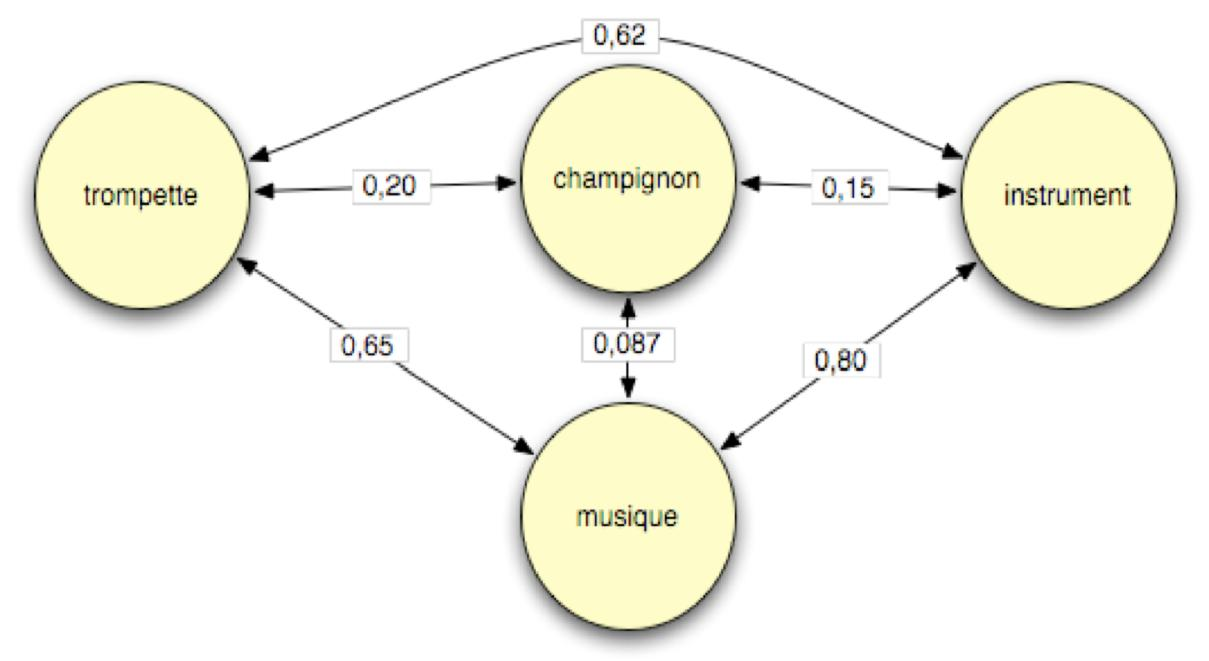
\includegraphics[width=0.75\textwidth]{img/lsa.jpeg}
    \caption[Caption for LOF]%
      {Un example de la LSA appliquée à quatre mots\footnote{PtiClic et PtiClic-kids~: Jeux avec les mots permettant une double acquisition. In proc TICE 2010, 7e coloque TICE, Nancy~: 6-8 décembre 2010}}
  \end{minipage}
\end{figure}


La LSA est plus fiable lorsque les textes utilisés pour générer les poids de relations sémantiques sont des corpus spécialisés. C'est une méthode rapide, facile à réaliser, efficace. Les données récoltées rélèvent en général de la langue écrite et donc un niveau de langue soutenue et riche. Un tel corpus contient une grande quantité de vocabulaire passif.

Il est plus difficile de se servir de la LSA pour des textes généralistes car elle ne traite pas la polysémie. Si l'on souhaite étudier la langue parlée, il faudrait des corpus qui sont des transcriptions de discours oraux. 

Les inconvénients de la LSA sont nombreux. Outre le fait qu'elle n'aborde pas le problème de la polysémie alors qu'en moyenne un mot donné a quatre significations différentes, lorsqu'il s'agit de textes écrits, les mots les plus courants et les plus évidents sont souvent omis~; les rédacteurs préfèrent utiliser des mots plus recherchés ainsi qu'éviter la répétition afin de conserver un bon style. Ceci va à l'encontre des statistiques sur les poids des relations entre les mots.\footnote{Ceci n'est pas vrai si les types de textes utilisés correspondent exactement aux types de textes auxquelles le résultat de la LSA est appliquée.} La LSA ne nous donne aucune information sur la syntaxe ni la morphologie des mots. Elle ne nous donne aucune information sur la nature des relations (synonymie, contenant/contenu, etc.). Enfin, la LSA traite chaque mot séparément. Autrement dit, chaque mot d'un mot composé est traité individuellement et confondu avec des occurrences individuelles de ces mêmes mots.

Malgré ces inconvénients, malgré des 'erreurs' produites par la LSA, elle est utilisée aujourd'hui car elle nous donne beaucoup d'informations sémantiques justes concernant la relation entre les mots d'un corpus. 

\subsubsection{Le réseau lexical JeuxDeMots}

Etant donné la complexité du signe linguistique, l'idée d'associer à un signe linguistique plusieurs liens sémantiques est très intéressante. Bien que cela croisse la complexité de nos applications, ce choix est tout à fait justifié. On se rend compte que les définitions et les résultats des dictionnaires classiques et de synonymes et antonymes sont insuffisant et ne nous donnes que des informations limités concernant la valeur sémantique d'un mot, surtout qu'elle nous donne peu ou pas d'informations sur la valeur sémantique qu'entretiennent deux mots donnés. En effet, le fait même d'avoir des données concernant plusieurs types de relations existant entre différents mots nous donne des informations supplémentaires quant aux connotations et aux dénotations d'un mot donné que celles d'un dictionnaire classique.

\begin{figure}
 \begin{minipage}{\textwidth}
\centering 
       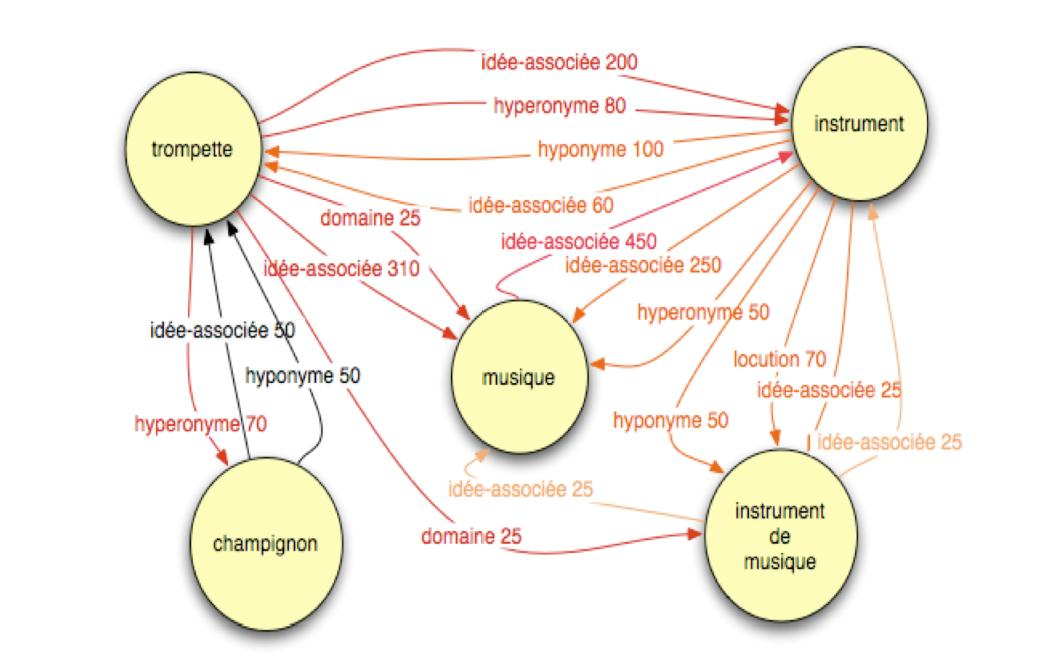
\includegraphics[width=0.75\textwidth]{img/jdm.jpeg}
    \caption[Caption for LOF]%
      {Un example des relations sémantiques du réseau lexical JeuxDeMots appliqué à quatre mots\footnote{Lafourcade et Zampa, PtiClic et PtiClic-kids~: Jeux avec les mots permettant une double acquisition. In proc TICE 2010, 7e coloque TICE, Nancy~: 6-8 décembre 2010}}
  \end{minipage}
\end{figure}

A l'inverse de la LSA, le réseau lexical JeuxDeMots est un réseau basé largement sur un vocabulaire actif composé de relations générales, le vocabulaire relevant plutôt de la langue orale créé de manière spontanée par des utilisateurs jouant au jeu. Ce réseau traite la polysémie, contient un grand nombre d'informations concernant les entrées morphologiques, syntaxiques et sémantiques voire pragmatiques. 

Les inconvénients sont que ces informations peuvent contenir des bruits et des silences.\footnote{Lafourcade et Zampa, PtiClic: A Game for Vocabulary Assessment Combining JeuxDeMots and LSA. In proc of CICLingj(Conference on Intelligent text processing and Computational Linguistics). Mexico, 1-7 March, 2009}. Des bruits sont des associations imprécises, qui en général doivent être plus faibles. Ceci peut arriver lorsque les réponses attendus sont celles correspondant au sens propre d'un mot alors que l'utilisateur donne un sens figuré ou bien fait de l'humour, après tout, il s'agit bien d'un jeu. L'exemple du mot poésie par exemple et l'association "est lié à" peut donner lieu à des réponses de sens propre ('auteur', 'rhyme', etc.) ou de sens figuré ('symphonie', 'amour', etc.). L'autre inconvénient est que le réseau JeuxDeMots contient un grand nombre de silences. Un 'silence' est défini comme une association n'existant pas ou qui devraient être plus forte. En effet, les informations sémantiques du réseau JeuxDeMots sont très hétérogènes et pas représentatif de la réalité alors que la LSA est plus hétérogènes quant à sa relation aux textes utilisés pour sa génération. 

Le réseau lexical permet aussi de générer un graphe donnant un seul arc entre deux mots similaire au graphe créer par la LSA. L'algorithme se déroule comme suit~:

\begin{figure}
 \begin{minipage}{\textwidth}
\centering 
       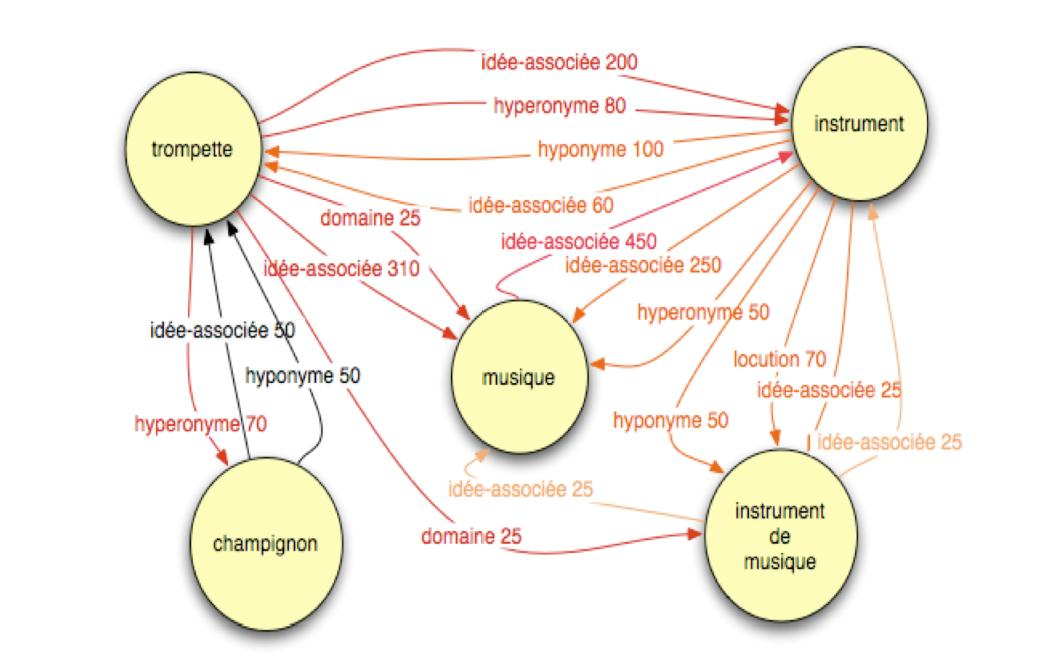
\includegraphics[width=0.75\textwidth]{img/jdm.jpeg}
    \caption[Caption for LOF]%
      {Un example des relations sémantiques du réseau lexical JeuxDeMots appliqué à quatre mots\footnote{Lafourcade et Zampa, PtiClic et PtiClic-kids~: Jeux avec les mots permettant une double acquisition. In proc TICE 2010, 7e coloque TICE, Nancy~: 6-8 décembre 2010}}
  \end{minipage}
\end{figure}


1. Pour un mot M (par exemple, 'musique') en relation avec un terme T (par exemple, 'instrument'), on additionne les relations entrantes et sortantes pour obtenir le 'poids' de la relation, ce poids est calculé pour tous les termes en relation avec le mot M.

\begin{center}
        \begin{tabular}{ | l | l | l | p{5cm} |}
        \hline
        Relation M-T & Calcul du poids & Poids \\ \hline
        musique-instrument & 450+250+50 & 750 \\ \hline
        musique-trompette & 310+25 & 335 \\ \hline
        musique-instrument de musique & 25 & 25 \\
        \hline
        \end{tabular}
\end{center}

2. On normalise cet ensemble comme suit~:

N = \[ 
\sqrt{((poids (musique-trompette))^2 + (poids (musique-instrument))^2 + (poids (musique-instrument de musique))^2} 
\]

= 
\[
\sqrt{(335^2 + 25^2 +750^2)}
\]

 =  
\[ 
\sqrt{(112225 + 625 + 562500)} 
\]

= 822

3. On calcule la signature. La signature S de Musique, c'est-à-dire S(Musique) est calculée comme suit~:

S(musique)~: \\
musique-instrument = 750/822 = 0.91 \\ 
musique-trompette = 335/822 = 0.40 \\
musique-instrument de musique = 25/822 = 0.03 \\

Les valeurs ainsi calculées donnent des résultats assez proches de ceux de LSA.


\subsection{Analyse pour la réalisation du projet PtiClic sous Android et Smartphone}

Toute la discussion précédente concernant PtiClic et le TALN à l'exception de l'algorithme décrit précédemment était une discussion d'ordre général concernant la raison d'être des projets JeuxDeMots et PtiClic. Le partie qui suit concerne des idées, des informations et des algorithmes directement liés à la réalisation du présent projet. 

L'introduction de nouvelles relations mettant en jeu des noeuds n'ayant aucune relation sémantique associée ne sera pas abordée car nous n'avions pas les moyens de mettre en oeuvre de tels procédés et un tel travail va au-delà du sujet du présent TER.\footnote{Une discussion concernant ce sujet a eu lieu avec Monsieur Lafourcade, qui nous a indiqué clairement de ne pas nous occuper de ce problème précis}  

Dans ce qui suit, 'mc' signifie 'mot central' et 'mn' signifie 'mot nuage'.

Les onze relations qui sont dans la version originale du jeu impose les contraites de catégories grammaticales suivantes~:




\begin{center}
        \begin{tabular}{ | l | l | l | p{5cm} |}
        \hline
        Relation M-T & Calcul du poids & Poids \\ \hline
        musique-instrument & 450+250+50 & 750 \\ \hline
        musique-trompette & 310+25 & 335 \\ \hline
        musique-instrument de musique & 25 & 25 \\ \hline
        \end{tabular}
\end{center}

\begin{center}
        \begin{tabular}{ | l | l | l | l | p{5cm} |}
        \hline
RELATION &	'mc' & 'mn'	& 'remarques' \\ \hline
-1 => "'mn' n'est pas lié à 'mc'" &	adj, adv, noms, verbes & adj, adv, noms, verbes	& \\ \hline
0 =>  "'mc' est en rapport avec 'mn'" & adj, adv, noms, verbes & adj, adv, noms, verbes & \\ \hline
5 => "'mc' est un synonyme de 'mn'" & adj, adv, noms, verbes & adj, adv, noms, verbes & même POS \\ \hline
6 => "'mc' est une sorte de 'mn'" & noms & noms & \\ \hline
7 => "Un contraire de 'mc' est 'mn'" & adj, adv, noms, verbes &	adj, adv, noms, verbes & même POS \\ \hline
8 => "Un spécifique de 'mc' est 'mn'" & noms & noms & \\ \hline
9 => "'mn' est une partie de 'mc'" & noms & noms & \\ \hline
10 => "'mc' fait partie de 'mn'" & noms & noms & \\ \hline
13 => "Quoi/Qui pourrait 'mc'" & verbes & noms & \\ \hline
15 => "Le lieu pour 'mc' est 'mn'" & noms, verbes & noms (lieu NON!!) & \\ \hline
16 => "Un instrument pour 'mc' est 'mn'" & verbes & noms & \\ \hline
17 => "Un caractéristique de 'mc' est 'mn'" & noms & adj & \\ \hline
        \end{tabular}
\end{center}

Les relations 5 et 7, la synonymie et l'antonymie, bien qu'elle peuvent être de plusieurs catégories grammaticales différentes, doivent contenir un mot central et des mots nuages de la même catégorie grammaticale alors que la relation 0, par exemple, peut avoir un mot central d'une catégorie grammaticale et des mots nuage de plusieurs différentes catégories grammaticales. Le relations 6 et 8, 9 et 10 doivent être des substantifs et ainsi de suite.

Remarquez qu'il ne suffit pas de choisir un mot nuage de la bonne catégorie grammaticale. Par exemple, dans la relation 16, les mots nuages potentiels doivent non seulement être des substantifs, mais doivent aussi être des choses. Le mot 'beauté' est un substantif mais ne sera pas un candidat mot nuage pour la relation 16. 

Il est plus intéressant de créer le nuage à partir de la relation 0 et d'introduire des relations plus spécifiques, c'est-à-dire n'importe quelle relation à l'exception de la relation 0, car presque toute relation est un sous-ensemble de la relation 0, la relation d'antonymie étant parfois une exception à la règle. 

L'isolation d'une seule relation permet d'établir si oui ou si non un mot est lié à un autre mot. Lorsqu'il y a deux ou plusieurs relations, le fait qu'un mot peut appartenir à un seul relation diminue le nombre de fois qu'un mot sera inclu dans une telle relation. 

Certaines relations sont incompatibles. Par exemple, la relation 13 doit avoir comme mot central un verbe alors que la relation 17 doit avoir comme mot central un nom. Si une partie est composée uniquement de la relation 13 et la relation 17, il est évident qu'une des relations n'aura aucune réponse possible car elle sera dépourvue de sens. Un autre exemple d'incompatibilité est dans le relation nuage. Si une partie contient seulement les relations 10 et 17, qui ont toutes les deux comme mot central un substantif, il serait possible de déduire à partir de la catégorie grammaticale quels mots sont candidats aux relations en question~: seuls les adjectifs sont candidats à la relation 17, seuls les noms sont candidats à la relation 10. Il serait intéressant de sanctionner plus sévèrement un utilisateur qui fait ce genre d'erreur lors d'une partie. 

Les relations 5 et 7 vont bien ensemble car elles contiennent exactement les même possibilités de POS comme mots central et nuages. En outre, les relations synonyme/antonyme sont antonymique, donc, il est rare que deux réponse soit possible, bien que la polysémie peut donner lieu à une exception (par exemple, le mot 'terrible' peut être synonyme ou antonyme à la fois de 'très bien' et de 'très mauvais'). Si l'on combine ces relations avec d'autres relations, il faudrait vérifier que les POS correspondent. Par exemple, 5, 7, 8, 9 et 10 peuvent être combiné pourvu que les relations 5 et 7 n'utilise que des noms.

Lorsque l'on trouve un moyen d'introduire de nouvelles relations tels que la LSA, il serait intéressant dans un premier temps d'introduire un mot central, des mots nuages et uniquement la relation 0. Ensuite, les données récupérées à partir de ce procédé pourraient utiliser pour raffiner ces relations. c'est-à-dire, à un mot central C et des mots nuages $N_{1}$ à $N_{n}$ qui ont été liés à C par la relation C, on prend ce même mot central et on introduit des relations autre que la relation 0. 


BOOKMARK
\subsection{*****CE QUI SUIT A ETE REDIGE IL Y A QUELQUE TEMPS ET DOIT ETRE RELU, DEVELOPPE, SUPPRIME OU INTEGRE AU TEXTE CI-DESSUS****}

\subsubsection{Quelles relations mettre ensemble~? Quelles relations seraient en conflit~?}

\subsubsection{La relation 0}
La relation 0, r\_associated, "\%mn n'est pas lié à \%mc", est très générale et presque toute relation peut aussi être ajoutée à cette relation. Un synonyme a aussi "un rapport avec", un "instrument pour" a aussi "un rapport" avec. La seule exception qui pourrait parfois s'y produire est la relation d'antonymie, mais même là, elle pourrait bien avoir un rapport avec (froid/chaud, chat/chien). Pour cette raison, puisque il est plus intéressant de produire des relations plus spécifiques pour affiner les liens sémantiques, et étant donné que les mots issues de JDM ont été généré à l'aide de cette relation, il n'y a que deux cas où cette relation est intéressante~: 

- pour générer le nuage afin de mettre les mots de cette relation dans des relations plus spécifiques
- d'introduire des mots issus de LSA dans cette relation pour ensuite pouvoir affiner à l'aide du point précédent

\subsubsection{Nombre de relations}
Il serait intéressant de varier le nombre de relations. Avoir une seule relation (plus la relation "poubelle") permet d'isoler une seule relation. Il s'agit d'un 'oui' ou 'non' et on élimine la possibilité qu'un mot n'est pas affecté à une relation à cause du fait qu'il irait potentiellement dans deux relations différentes. 

Puis, certains relations sont directement lié et présente aucun conflit. Par exemple, la relation d'antonymie et de synonymie sont elle-même antonymique et prennent les mêmes types de mots (POS) en tant que mots nuages et mot central. Aucun conflit pourrait y arriver si tout mot est de la méme POS.  


\subsubsection{Des relations en conflit à cause du POS}
Certaines relations seraient en conflit si combiner~: Il n'est pas possible de combiner la relation 16 et la relation 17 car le mot central de la relation "Un instrument pour \%mc est \%mn" prend comme mot central un verbe et la relation "Un caractéristique de \%mc est \%mn" prend comme mot central un nom. En outre, les mots nuages correspondants ne sont non plus du même POS~: la relation 16 prend comme mot nuage un nom alors que la relation 17 prend comme mot nuage un adjectif. 

De même, même si un mot central prenait un mot de même POS, si les mots nuages étaient obligatoirement de POS différents, cela faciliterait la tâche du joueur, qui, consciemment ou non, pourrait "tricher" en sachant qu'une des relations prend un nom alors que l'autre prend un adjectif. C'est le cas de la relation 8, 9 et 10 qui ont comme mots central et nuages un nom et la relation 17 qui elle aussi a comme mot central un nom mais qui prend obligatoirement un adjectif comme mot nuage. Ces relations devraient jamais être combinées, ou bien, ce serait intéressant de pénaliser un jour davantage lorsqu'il se trompe de POS attendu. 



Bien sûr, il est tout à fait possible de mélanger des POS en ayant 3 ou 4 relations et pour tester la légitimité des réponses des joueurs et leur fiabilité, mais cela rend en quelque sorte plus facile au joueur de jouer, quoique tout mot ne va pas forcément dans une catégorie, il existe aussi des mots poubelles, mais cela fournit une aide tout de même pour le joueur, s'il peut savoir à 100\% qu'un mot ne peut pas correspondre à une relation à cause de sa catégorie grammaticale. 



\subsubsection{POS correct, mais conflit tout de même~!}
Il peut arriver dans une relation qu'on a les bonnes catégories grammaticales dans les mots nuages, mais que les mots nuages sont inappropriés pour la relation en question. 

Par exemple, pour la relation "Quoi/Qui pourrait \%mc", la relation 13, il ne suffit pas que le mot nuage soit un nom, loin de là~!. Le substantif "honnêteté" ne convient pas du tout~! Il faudrait aussi exploiter d'autres ressources de la base de données, par exemple, un substantif qui est aussi un métier ou une personne ou un animal.

Ou bien, pour la relation partie/tout, il faut absolument que la chose soit un objet physique, une chose. 

Nuage noms -> 6, 8, 9, 10, 13, (15 .. LIEU), 16 (à vérifier)

Noms/choses -> 6, 8, 9, 10 (à vérifier)



TODO~: 

\subsubsection{Relations qui pourraient être ajoutées au jeu (car lien avec la sémantique)}
TODO: lister, développer

\subsubsection{Relations qui ne pourraient pas être ajoutées au jeu (car aucun lien avec la sémantique)}
Liste avec brièves explications

?? des moyens de contourner les problèmes liés au problème de relation à l'aide de la relation 'est de la même famille' et des expressions régulières, etc.~??



\subsubsection{Algorithmes pour affiner ou renforcer des relations déjà existantes}

Les algorithmes ci-dessous serait potentiellement générateur de nouvelles relations. Ce ne sera pas toujours le cas à cause de la polysémie et le fait que différents mots ont différentes nuances de signification. Il faudrait tester les algorithmes pour savoir ce qu'ils donnent. Il faudrait toujours vérifier que le mot obtenu par ces algorithmes ne produisent pas le mot de départ, de vérifier que le résultat est différent que le ou les mots passés en paramètre. 

\subsubsection{Relation 0 - "\%mn n'est pas lié à \%mc"}
A ne pas utiliser pour cette fin. Seulement comme indiquer ci-dessus, je répète ici: 
- pour générer le nuage afin de mettre les mots de cette relation dans des relations plus spécifiques
- d'introduire des mots issus de LSA dans cette relation pour ensuite pouvoir affiner à l'aide du point précédent

\subsubsection{Relation 5 - "\%mc est un synonyme de \%mn"}

- un synonyme d'un synonyme pourrait être un synonyme, ainsi qu'un synonyme d'un synonyme d'un synonyme
- un antonyme (relation 7) d'un antonyme pourrait être un synonyme, ansi qu'un antonyme d'un antonyme d'un antonyme  d'un antonyme (Bonjour~!) 

\subsubsection{Relation 6 - "\%mc est une sorte de \%mn"}
- "Une moto est une sorte véhicule" où "moto" est le mot central et "véhicule" est un parmi plusieurs mots nuages. L'algorithme va partir de "moto" pour trouver "véhicule" ou bien "deux roues" (relation 6), puis faire marche arrière (relation 8, "Un spécifique de \%mc est \%mn"), par exemple, un spécifique "véhicule" est "voiture" ou bien un spécifique de "deux roues" est "vélo". Ensuite, on génère la relation "sorte de" à partir de ce résultat... "voiture" est une sorte de "moyen de transport" ou bien "vélo" est un "équipement de loisir". Le résultat final~: "moto" est-elle un "moyen de transport"~? "moto" est-elle un "équipement de loisir"~? 
En somme, on effectue la relation 6, la relation 8 puis la relation 6 encore.  

\subsubsection{Relation 7 - "Un contraire de \%mc est \%mn"}
- un synonyme d'un antonyme pourrait être un antonyme
- un antonyme d'un synonyme pourrait être un antonyme
- un antonyme d'un antonyme d'un antonyme pourrait être un antonyme (Bonjour~!)


\subsubsection{Relation 8 - "Un spécifique de \%mc est \%mn"}

- C'est l'inverse de la relation 6. On effectue la relation 8, puis la relation 6, puis la relation 8.


\subsubsection{Relation 9 -  "\%mn est une partie de \%mc"}
- "salon" est une partie de "maison". On peut choisir un spécifique de "maison" et ensuite effectuer la relation 9. Si spécifique nous donne "église", il y a des parties de l'église qui sont commune aux parties d'une maison, d'autres qui sont spécifiques à "église".
- On peut également basculer de la partie vers le tout puis encore vers la partie
- On peut trouver la partie d'une partie, puis le tout de cette dernière.
- On peut trouver le tout du mot central "maison" fait partie de "ville", une partie de cette dernière ("ville"), puis encore une partie de cette dernière.  


\subsubsection{Relation 10 - "\%mc fait partie de \%mn"}
- il s'agit de l'inverse de la relation 9. Il suffit d'effectuer les étapes inverses aux algorithmes de la relation 9



\subsection{CONCLUSIONS}
Il est intéressant que lorsque l'on fait une recherche dans ce domaine, on apprend énormément de choses de la machine, puis à partir des choses apprises, on modifie le fonctionnement de la machine, qui elle, nous fournit encore des résultats, et ainsi de suite. La machine apprend de nous et nous, nous apprenons de la machine. C'est un vrai dialogue~! ... 








\section{Conception}


\subsection{Base de données}

Le schéma relationnel suivant a été modélisé à partir des informations du dump de la base de données d'origine et nos besoin en matière d'authentification et de sécurité côté serveur~:

TODO : A METTRE A JOUR, PLUS D'ACTUALITE

{\footnotesize
NODE(\underline{EID}, name, \#type, weight) \\ 
RELATION(\underline{RID}, \#start, \#end, \#type, weight) \\
TYPE\_NODE(\underline{num}, name) \\
TYPE\_RELATION(\underline{num}, name, extended\_name, info) \\
USER(\underline{login}, mail, hash\_passwd, \#score) \\
GAME(\underline{GID}, \#eid\_central\_word, \#relation\_1, \#relation\_2, difficulty) \\
GAME\_CLOUD(\underline{GID, num}, difficulty, \#eid\_word, totalWeight, probaR1, probaR2, probaR0, probaTrash) \\
PLAYED\_GAME(\underline{PGID}, \#gid, \#login) \\
PLAYED\_GAME\_CLOUD(\underline{\#PGID, \#GID, num}, type, \#relation, weight, score) 
}

Si nous reprenons nos deux petits exemples d'entrées NODE et RELATION du dump de la base de données, il devient clair que les tables NODE et
RELATION y correspondent strictement à la structure d'origine~: \verb!eid=231064:n="pour femme":t=1:w=50!, où «eid» correspond à «EID», $n$ à
«name», $t$ à «type» et $w$ à «weight» de la table NODE de notre base~; \verb!rid=430049:n1=82029:n2=151553:t=12:w=18! où $rid$ correspond à «rid»,
$n_1$ à «start», $n_2$ à «end», $t$ à «type» et $w$ à «weight» de la table RELATION de notre base.



TYPE\_NODE(\underline{num}, name) \\

%// ---- Node stats

%/// 3 occurrences of nodes n_generic (t=0)
%/// 228800 occurrences of nodes n_term (t=1)
%/// 0 occurrences of nodes n_acception (t=2)
%/// 0 occurrences of nodes n_definition (t=3)
%/// 143 occurrences of nodes n_pos (t=4)
%/// 1001 occurrences of nodes n_concept (t=5)
%/// 42 occurrences of nodes n_flpot (t=6)
%/// 0 occurrences of nodes n_hub (t=7)
%/// 17 occurrences of nodes n_data (t=18)
%/// 39 occurrences of nodes n_data_pot (t=36)
%/// 956 occurrences of nodes AKI (t=666)

TYPE\_RELATION(\underline{num}, name, extended\_name, info) \\

???

%*************
%NE PAS EFFECER -> CI-DESSOUS LE SCHEMA COMME DECRIT PAR GD 

%NODE(EID integer primary key autoincrement, name string, #type (ref TYPE_NODE.num), weight);
%RELATION(RID integer primary key autoincrement, #start (ref NODE.eid), #end (ref NODE.eid), #type (ref %TYPE_RELATION.num), weight);
%TYPE_NODE(NUM, name string);
%TYPE_RELATION(NUM, name string, extended_name string, info string);
%USER(LOGIN string primary key, mail string, hash_passwd string (md5sum du password), #score (contrainte : somme de tous les scores des PLAYED_GAME_CLOUD);
%GAME(GID integer primary key autoincrement, #eid_central_word (ref NODE.eid, #relation_1 (ref RELATION.rid), #relation_2 ( (ref RELATION.rid), difficulty (contrainte : 10 <= difficulty <= 100));
%GAME_CLOUD(GID, NUM, difficulty (contrainte : 1 <= difficulty <= 10), #eid_word(ref NODE.eid), totalWeight (contrainte : = somme des probas), probaR1 (contrainte : = somme des probas des PLAYED_GAME_CLOUD.weight avec la bonne relation et la même gid et num), probaR2 (idem), probaR0 (idem), probaTrash (idem));
%PLAYED_GAME(PGID integer primary key autoincrement, #gid (ref GAME.gid), #login (ref USER.login);
%PLAYED_GAME_CLOUD(#PGID (ref PLAYED_GAME.pgid), #GID (ref PLAYED_GAME.gid), NUM, type (contrainte : 0 = partie de référence, 1 = réponse d'un joueur), #relation (ref RELATION.rid), weight (contrainte : probabilité estimée de cette réponse pour les bots (robots), réputation du joueur sinon), score (score donné au joueur, 0 pour les bots);

%**INT unless otherwise marked

%create table node(eid integer primary key autoincrement, name, type, weight);
%create table relation(rid integer primary key autoincrement, start, end, type, weight);
%create table type_node(name, num);
%create table type_relation(name, num, extended_name, info);
%create table user(login primary key, mail, hash_passwd, score);
%create table game(gid integer primary key autoincrement, eid_central_word, relation_1, relation_2, difficulty);
%create table game_cloud(gid, num, difficulty, eid_word, totalWeight, probaR1, probaR2, probaR0, probaTrash);
%create table played_game(pgid integer primary key autoincrement, gid, login);
%create table played_game_cloud(pgid, gid, type, num, relation, weight, score);

%create index i_relation_start on relation(start);
%create index i_relation_end on relation(end);
%create index i_relation_type on relation(type);
%create index i_relation_start_type on relation(start,type);
%create index i_relation_end_type on relation(end,type);

TODO: UML, diagrammes de classes, Use cases, etc.

\subsection{Site Internet}
% TODO : Yoann
Afin de pouvoir utiliser le jeu il faut posséder un compte utilisateur. Un utilisateur qui installe pour la première fois l'application sur son smartphone devra obtenir un compte avant de profiter du jeu.

Le site Internet permet de réaliser cette inscription grâce à un formulaire qui permet la saisie des informations nécessaires. Il est également un moyen de présenter le projet, l'application et de prendre contact avec les développeurs.

Le site est constitué d'un petit nombre de pages à savoir : une présentation de l'application et du projet, l'inscription et l'authentification, une page de téléchargement de l'application et de procédure d'installation, ainsi que quelques pages permettant de créer et afficher des parties.

Les deux dernières pages citées concernant la création et l'affichage de parties ne sont pas accessibles à tout le monde. Il faudra que l'utilisateur débloque ce mode en obtenant un certain nombre de points dans le jeu.

\subsection{Site Internet 2}
Le site Internet est en grande partie "statique" (langage HTML). Les pages "statiques" sont les pages de présentation, de contact et de téléchargement.

Certain éléments comme l'inscription, la connexion\dots{} ont une partie PHP qui permet d'intérroger la base de données afin de valider ou non l'action.

La création de parties est, elle, réalisée en PHP et JavaScript afin de rendre plus intuitif l'interraction avec l'utilisateur. Les parties générées par les utilisateurs sont ajoutées dans la base de données pour qu'elle puissent par la suite être jouées par les autres joueurs. Le nom de la personne ayant créer la partie est associé à celle-ci ce qui permettra d'indiquer aux joueurs la personne qui à créer la partie à laquelle il sont entrain ou ils viennent de jouer. Par soucis de maintien d'une base de donnée propre, l'utilisateur ne peux pas rentrer de nouveaux mots dans la base de données. Lorsqu'il souhaite créer une nouvelle partie il doit utiliser des mots "connus". Le JavaScript permet de vérifier dynamique la validité des mots et ainsi indiquer immédiatement à l'utilisateur si le mot qu'il vient saisir est correct ou non.

\subsection{Version html5 du jeu}
\label{sec:html5}
\subsubsection{Architecture}

La version HTML5 du jeu est architecturée de la manière suivante~:

L'application comporte 6 écrans~:
\begin{itemize}
\item Le «splash» au démarrage;
\item L'éran d'accueil, avec des liens vers les 4 autres (sauf score);
\item L'écran du jeu, avec le mot central, le mot du nuage et les quatre relations;
\item Le score, affiché à la fin de la partie;
\item Les préférences, qui permettent de choisir le thème de couleurs de l'application;
\item L'écran de connexion, sur lequel on peut se rendre depuis l'écran d'accueil, et qui s'affiche automatiquement lorsqu'on tente de faire
  une action (jouer ou modifier les préférences) sans être connecté;
\item L'écran «À propos», qui explique l'origine du jeu.
\end{itemize}
Chaque écran est contenu dans un élément HTML (\verb!<div/>!) qui est affiché uniquement lorsque l'utilisateur est sur cet écran.

La navigation entre les écrans, et entre chaque mot du nuage lorsqu'on joue à la partie, s'effectue en modifiant l'identifiant de fragment
de l'URL (la partie après le \verb!#!). De cette manière, chaque état est stocké dans l'historique du navigateur, et on peut revenir à
l'écran précédent en utilisant les botons «Précédent» et «Suivant» classiques. De plus, cela permet d'annuler le choix d'une relation pour
un mot donné simplement en cliquant sur «Précédent».

L'état du programme (écran en cours, thème de couleurs, structure de données représentant la partie en cours lorsqu'elle a été récupérée,
même chose pour les scores) est stocké dans une variable nommée \verb!runstate!. Cependant, si l'on considère l'enchaînement d'actions
suivantes, on se rend compte qu'il doit y avoir une décorrélation entre l'état du programme tel que dicté par l'URL, et l'état réel du
programme~:
\begin{itemize}
\item L'utilisateur clique sur «Jouer», ce qui l'amène à l'URL \verb!#game!;
\item L'écran de connexion est affiché pour que l'utilisateur s'identifie, sans modifier l'URL (pour ne pas enregistrer cette étape
  transitoire dans l'historique).
\item Une fois que l'utilisateur est connecté, la partie commence.
\end{itemize}
Cette décorrélation apporte une certaine complexité au code de transition entre les états du programme, d'autant plus que l'application
effectue des requêtes réseau asynchrones, par exemple pour récupérer la partie, durant lesquelles n'importe quelle séquence de «Précédent» /
«Suivant» ou de modifications arbitraire peut avoir lieu. Ainsi, entre le moment où on effectue une requête pour récupérer une nouvelle
partie, et le moment où cette requête aboutit, l'utilisateur peut avoir cliqué sur «Précédent», ce qui le ramène à l'écran d'accueil (auquel
cas il ne faut pas afficher la partie lors de la réception), mais il peut aussi après ce «Précédent» faire «Suivant», auquel cas on se
retrouve de nouveau sur l'écran du jeu, et il faut donc afficher la partie lors de sa réception (et ne pas faire une deuxième requête
puisqu'il y en a déjà une en cours).

Pour gérer cela, nous avons implémenté une routine de transition entre les états, qui envoie la séquence de messages suivante au nouvel
écran~:
\begin{itemize}
\item «goto», qui envoie le message «leave» à l'écran en cours, met à jour la variable runstate.screen, et communique quelques informations
  à l'application hôte en Java sous Android;
\item «pre-enter», qui permet à l'écran d'effectuer des requêtes réseau avant son affichage;
\item «enter», qui affiche l'écran, et modifie dynamiquement son contenu si nécessaire (par exemple affichage du texte décrivant les
  relations dans l'écran du jeu);
\item «update», appellée une première fois juste après l'affichage de l'écran, et à chaque changement d'URL qui ne modifie pas l'écran. Cela
  permet par exemple à l'écran du jeu de détecter qu'une réponse a été donnée pour un des mots du nuage, et d'afficher le mot suivant.
\end{itemize}

Un changement d'URL déclenche donc soit un «goto», soit un «update», ce qui permet d'afficher l'écran voulu, tandis que les écrans peuvent
s'envoyer les uns les autres ces messages (principalement le message «goto») pour basculer de l'un à l'autre sans modifier l'URL.

\subsubsection{Concepts et techniques de programmation}

Les actions à déclencher lors de la réception du résultat d'une requête réseau, ainsi que le cache partiel des parties et des scores (qui
permet de ne pas renvoyer une requête qui est déjà en cours ou a déjà abouti), sont implémentés en utilisant le paradigme de programmation
fonctionelle avec évaluation paresseuse, le côté «évaluation paresseuse» étant émulé en encapsulant le code dans des fonctions anonymes
(lambda fonctions).

Nous avons aussi employé une forme limitée de programmation réactive pour le cache, implémentée via l'objet \verb!Deferred! de jQuery.

Enfin, nous avons utilisé les capactités de javaScript lui-même, qui est un langage objet basé sur les prototypes (et non les classes), pour
étendre le langage là où cela s'est avéré nécessaire.

\section{Réalisation}
\subsection{Cahier des charges}

\subsection{Cahier des charges initial}
Avant le début du projet, nous avions planifié l'implémentation des fonctionnalités souhaitées de notre application. Le déroulement du
travail devait s'effectuer sur 4 itérations, décrites ci-dessous.

Chaque itération comprenait 2 semaines pour implémenter les fonctionnalités, une semaine pour d'éventuelles améliorations ou pour
implémenter des détails que nous n'aurions pas eu le temps d'implémenter, et une semaine pour corriger les bugs signalés lors des
alpha-test. Après chaque itération, nous devions livrer une version stable aux alpha-testeurs, pour un alpha-test de 2 semaines.

\begin{itemize}
\item Itération 1
  \begin{itemize}
  \item Serveur capable de générer les parties (choix du mot central et des mots du nuage).
  \item Application \android{} qui récupère une partie, et permet d'y jouer.
  \item Gestion des logins/mot de passe.
  \end{itemize}
\item Itération 2
  \begin{itemize}
  \item Ajout de niveaux de difficulté sur les parties.
  \item Mode «Marathon»~:faire la plus longue parties possible avec un maximum de $n$ fautes.
  \item Mode «Shoot'em up»~:Une seule relation, et tous les mots du nuage affichés en même temps. L'utilisateur doit cliquer sur les mots
    qui appartiennt à cette relation puis indiquer qu'il a terminé. Ce mode est assez proche conceptuellement du fonctionnement original de
    PtiClic.
  \end{itemize}
\item Itération 3
  \begin{itemize}
  \item Thèmes pour l'apparence et pour des questions d'accessibilité~: modification des couleurs et des tailles des éléments.
  \item Intégration avec des réseaux sociaux, pour promouvoir l'application.
  \item Mode de jeu «Multijoueur»~: Deux joueurs jouent à la même partie, et leurs scores sont comparés.
  \end{itemize}
\item Itération 4
  \begin{itemize}
  \item Mode de jeu «Thématique»~: Après avoir choisi un thème (noël, informatique, \dots), on propose à l'utilisateur des parties avec des
    mots centraux reliés à ce thème.
  \item Mode de jeu «Chrono»~:une seule relation, les mots du nuage apparaissent et disparaissent assez rapidement, et il faut cliquer sur
    la relation uniquement pour les mots qui y appartiennent (le reste va implicitement à la poubelle). Ce mode nécessitait d'implémenter la
    possibilité de mettre en pause le jeu étant donné que le temps y a une importance.
  \item Interface vocale, pour améliorer l'accessibilité de l'application.
  \end{itemize}
\end{itemize}

Le diagramme de gantt en annexe \ref{sec:gantt-original} présente l'ordonancement et l'affectation des tâches de chacunes des itérations.

\subsection{Travail effectué}

L'itération 1 a pris plus de temps que prévu, en partie à cause des difficultés rencontrées \ref{sec:difficultes}, et aussi parce que nous
nous sommes rendus comptes que certaines fonctionnalités devaient être plus avancées avant que l'application soit livrée.

Entre autres, nous avons passé du temps à améliorer et régler les paramètres de l'algorithme de génération de parties, étant donné que
l'algorithme naïf prévu au départ donnait des résultats assez mauvais.

Nous avons aussi amélioré le serveur sur les points suivants~:
\begin{itemize}
\item Refus d'enregistrer les réponses pour une partie si elle a déjà été jouée (pour prévenir les tentatives de tricherie de la part des joueurs).
\item Protocole de transmission des erreurs entre le serveur et le client, par exemple lorsqu'un paramètre manque à la requête, ou lors d'un
  accès à une partie inexistante.
\end{itemize}

De plus, au départ, nous pensions fournir directement l'application aux alpha-testeurs, mais étant donné la nécessité d'avoir les noms d'utilisateurs
et mots de passe dans la base, il semblait peu avantageux de gérer ces points manuellement. Nous avons aussi dû créer un site web à destination
des utilisateurs, pour qu'ils puissent s'inscrire, télécharger l'application (avec des explications sur la procédure d'installation), et
s'informer sur le projet.

Ainsi, à la fin de l'itération 1, après envoi de la version aux alpha-testeurs, et après discussion avec notre tuteur, nous avons
radicalement changé le cahier des charges pour qu'il devienne le suivant~:
\begin{itemize}
\item Itération 1 (effectuée)
  \begin{itemize}
  \item Serveur robuste capable de générer les parties d'une qualité acceptable.
  \item Application \android{} qui récupère une partie, et permet d'y jouer, avec un écran permettant aux utilisateurs de configurer
    l'application (adresse du serveur, login et mot de passe).
  \item Gestion des logins/mot de passe sur le serveur et le client.
  \item Site web de présentation du projet.
  \end{itemize}
\item Itération 2
  \begin{itemize}
  \item Passage d'une version native à une version web, pour pouvoir toucher plus d'utilisateurs, et à cause des difficultés de l'environnement Android.
  \item Au lieu d'intégrer l'application à des réseaux sociaux, ajout d'un bouton «j'aime» ou «j'aime pas», et permettre aux joueurs d'avoir des «amis» etc.
  \item Outil de création manuelle de parties accessible aux joueurs sur le site, avec les extensions du serveur nécessaires.
  \item Pousser plus loin la recherche sur les méthodes de création de parties, et étude de la base du point de vue linguistique et TALN.
  \end{itemize}
\end{itemize}

Globalement, nous avons donc réduit le nombre de fonctionnalités à implémenter, tout en étoffant celles que nous avons conservé, afin
d'éviter d'avoir une application offrant une multitude de fonctionnalités qui seraient implémentées de manière superficielle.

\subsection{Langages}
Notre projet c'est découpé en 2 grosses parties. La première partie, la \og{}partie Serveur\fg{}, permet de réaliser des actions sur l'ensemble de la base de donnée (création de parti, validation de partie\ldots),
la réalisation de celle-ci c'est fait principalement en PHP, l'autre étant du SHELL.
La seconde partie, la \og{}partie Cliente\fg{}, permet à l'utilisateur de pouvoir intéragir avec le serveur, et surtout de pouvoir jouée à PtiClic. Elle à été réalisé en Java en utilisant le framework \android{} pour l'application mobile et avec le langage JavaScript pour l'application web.

\subsubsection{PHP}
Comme cité plus haut, nous avons utilisé PHP pour la création du serveur. PHP est un langage impératif, il dispose aussi depuis la version 5 de fonctionnalités objet, mais nous ne les utilisont pas dans notre projet. Ce langage est
principalement utilisé pour produire des pages Web dynamiques, c'est la raison de sont utilisation dans notre projet. C'est un langage peu typé, souple, multiplate-forme, libre et gratuit.
Nous utilisons donc PHP pour la création de notre site web \url{http://www.pticlic.fr} ainsi que pour toute la partie génération de partie à savoir la création, génération, envoie et récupération de partie PtiClic.

\subsubsection{SHELL}
Nous utilisons aussi le langage SHELL. Ce langage est surtout utilisé pour l'initialisation du serveur lors de sont installation sur un serveur différent. Son but, pour notre projet, et de récupérer le dernier dump (archive) de la base de donnée, de convertir ce dump en SQL et de l'insérer dans la base de donnée de type SQLite.

\subsubsection{SQLite3}
SQLite est une bibliothéque, écrite en C qui propose un moteur de base de données relationnelles accessible par le langage SQL. Contrairement aux serveurs de bases de donnée traditionnels, comme MySQL ou PostgreSQL, ça particularité est de ne pas reproduire le schéma habituel client-serveur mais d'être directement intégrée aux programmes. L'intégralité de la base de données est stockée dans un fichier indépendant de la plateforme. Le code source de SQLite est dans le domaine public, ce qui permet son utilisation sans restriction aussi bien dans les projets open source que dans les projet propriétaire.

\subsubsection{Java}
La partie cliente du projet est réalisé en Java. Ce langage est le plus utilisé dans le monde par les développeur. Java reprend en grande partie la syntaxe du langage C++. Néanmoins il a été épuré des concepts les plus déroutants du C++ tels que les pointeurs, les références, l'héritage multiples\dots{} La grande spécificité de ce langage est ça portabilité. En effet lors de la compilation, un bit code est généré, et celui-ci est ensuite lu par une machine virtuelle dépendante de la platforme.

\subsubsection{HTML5, JavaScript et jQuery}

La deuxième version de l'application, écrite en HTML5, utilise le langage JavaScript pour l'interaction avec l'utilisateur. La bibliothèque jQuery a été lourdement utilisée pour abstraire l'interface DOM (Document Object Model) fournie par le navigateur pour interagir avec le document HTML. Cette bibliothèque très extensible permet entre autres de manipuler facilement des collections entières d'éléments pour les modifier tous en même temps, de faire des requêtes complexes sur le document pour en récupérer une portion destinée à être manipulée, et
fournit aussi une couche d'abstraction pour les requêtes réseau asynchrones et la manipulation de données au format JSON (JavaScript Object Notation), qui est le format utilisé dans les échanges entre le client et le serveur. Dans le cadre de ce projet, nous avons été amenés à écrire plusieurs petites extensions à la bibliothèque jQuery, ce qui a été à chaque fois une tâche relativement aisée, vérifiant ainsi l'extensibilité de cette bibliothèque.

\subsection{Outils utilisés}
\subsubsection{Gestionnaire de versions~: Git et Github}

Pour synchroniser nos efforts sur le projet, nous avons utilisé le gestionnaire de versions distribué git, et hébergé notre projet sur la plate-forme github. Un des avantages d'un gestionnaire de version distribué par rapport à un gestionnaire de versions centralisé tel que SVN, est qu'il n'y a pas besoin d'un serveur central pour synchroniser deux copies du projet. Ainsi, nous avons pu partager nos modifications via une clé usb, même dans des lieux avec une connectivité réduite, comme la fac, où nous avons régulièrement travaillé. 
De plus, git possède un algorithme de résolution des conflits d'édition beaucoup plus efficace que celui de SVN, ce qui nous a permis de développer certaines fonctionnalités dans des branches séparées, et de les fusionner par la suite avec la branche principale, sans avoir à craindre une fusion manuelle des deux branches.

Une autre fonctionnalité appréciable de git est que chaque «clone» d'un dépôt conserve tout l'historique du projet, si bien qu'un crash du serveur n'impacte pas du tout le projet~: On met en place un autre serveur sur lequel on envoie une copie du projet, et tout fonctionne comme avant.

Nous avons choisi la plate-forme d'hébergement github pour la facilité de la mise en place d'un dépôt git (quelques clics suffisent), sa disponibilité élevée comparée à un serveur personnel, et parce que nous avions déjà utilisé cette plate-forme avec succès dans d'autres projets.

Github offre des fonctionalités supplémentaires telles que des graphes permettant de visualiser l'avancement du projet, un outil de rapport de bug et un wiki pour la documentation. Nous n'avons cependant pas utilisé ces deux dernières fonctionnalités, préférant un simple fichier texte pour garder une trace des bugs à corriger et des tâches à effectuer. Une des raisons motivant ce choix est qu'un des membres du groupe possède un ordinateur relativement peu performant et une connexion à Internet très peu fiable, qui rendent l'utilisation de ces services pénible (voire impossibles lors des fréquentes coupures du réseau).

\subsubsection{Environnement intégré de développement~: Eclipse}
Eclipse est un IDE extensible (par plugin) et polyvalent permettant de créer des projets mettant en oeuvre n'importe quel langage de programmation. Il est écrit en Java, et c'est avec ce langage que l'on peut créer de nouvelles extensions. La grande force de cet IDE est qu'il est développer autour des plugins pour pouvoir l'étendre.
Son choix d'utilisation vient aussi du faite qu'il est présent sur les ordinateurs de la faculté, et que nous avons l'habitude de l'utiliser.

\subsubsection{\android{}}
\android{} est un système d'exploitation open source pour smartphones. Pour ce TER nous avons donc utilisé le framework proposé par Google, pour le developpement d'application sur cet OS. Il est basé sur le langage Java, ce qui permet un apprentissage plus facile (du fait que ce langage est le plus utilisé dans le monde).

\paragraph{Software Development Kit (SDK)}
Le SDK d'\android{} posséde un grand nombre de classes et de paquetages sur l'ensemble des fonctionnalitées proposé par les périphèriques embarquant cet OS. On peut par exemple trouver un paquetage spécialisé dans les accès réseaux, bluetooth, d'autre pour la géolocalisation\dots{} Le developpement avec ce framework repose sur le modele (pattern en anglais) MVC (Model View Controller). Les modèles (du pattern MVC) sont principalement représenté avec des classes simple (héritant directement de \verb!java.lang.Object!). Les contrôlleurs eux hérite de la classe \verb!android.app.Activity! ou d'une de ces classes enfants. Quant aux vues, elles sont représenté avec un format XML.
La connexion entre les contrôlleurs et le vues est réalisé grâce à la methode \verb!public View findViewById (int id)! de la classe \verb!android.app.Activity!, qui parcours l'arbre XML pour récuperer l'objet correspondant à l'id passé en paramétre.

\paragraph{Developper Toolkit (ADT) Plugin}
L'ADT est un plugin développé par Google pour faciliter le developpement d'application \android{} avec Eclipse. Il propose un menu permettant de créer des projets de type \android{} déjà parametré selon les besoins. Mais aussi un gestionnaire d'emulateur, une disposition (au sens d'Eclipse) DDMS permettant de contrôler l'emulateur\dots{}

\section{Revirement des choix de developpement} % TODO : Devrait peut etre etre deplacé
A la fin de la première iteration, nous avons décidé de ne plus utiliser le système de création de vue proposé par le SDK d'\android{}, car, pour nous, la création de vue en passant par le format proposé nous prennait énormement de temps. \android{} supportant le framework WebKit ainsi que javascript dans son integralité et notre groupe ayant un peu plus d'expérience dans le développement d'application web (de part notre formation), nous avons décidé de développer les vues de l'application PtiClic en HTML5/Javascript. De ce faite, l'application à été simplifié (une seul Activité) et une classe \verb!JavascriptInterface! réalisant un pont entre le code javascript et les fonctionnalitées du téléphone à été ajouté.
Un autre avantage à l'utilisation d'une application web pour développer PtiClic est le publique visé. En effet, le but de ce jeu étant de récupère des données d'un grand nombres d'utilisateur, fournir l'application à d'autres personnes que celles disposant d'un smartphone sous \android{} nous a semblé interressante. C'est pourquoi avec la version 2 nous avons aussi une application jouable à partir d'un navigateur internet <<normal>>, ce qui permet à un plus grand nombres de personnes de pouvoir jouer à PtiClic.

\section{Discussion}
\subsection{Difficultés rencontrées}
\label{sec:difficultes}
\subsubsection{Itération 1, semaine 1}
\begin{itemize}
\item Outil de création de diagrammes de GANTT (planner) est assez mauvais.
\item Lenteur de l'émulateur \android{} : impossible de travailler sur mon PC.% gd
\item Caractères non échappés dans le dump de la base.% gd
\end{itemize}

\subsubsection{Itération 1, semaine 3}
\begin{itemize}
\item SQLite3 n'est pas capable d'utiliser un index pour la requête extérieure sur une requête du type

\begin{verbatim}
select * from (select * from table where condition) where condition
\end{verbatim}

Donc nécessité de ré-écrire certaines requêtes avec des jointures à priori beaucoup moins efficaces, mais qui le sont plus grâce aux index.
\item SQLite3 tranforme les requêtes de la forme~:

\begin{verbatim}
select * from table limit 100 order by random();
\end{verbatim}

  en une requête qui récupère tout le set de résultats, ajoute une colonne random(), prend les 100 premiers résultats et les trie. Mais cela
  l'oblige à récupérer tout le set de résultats, et calculer le random() pour chaque ligne, pour ensuite jeter tout ce qui dépasse la ligne
  100. Cela est évidemment très coûteux dans le cadre de requêtes avec beaucoup de résultats, et nous avons donc dû isoler la requête avec
  \verb!limit! de son \verb!order by! avec des «hacks» assez tordus.
\end{itemize}

\subsection{Perspectives}

Bien que fonctionnelle, notre application peut encore être améliorée. L'implémentation d'un des modes de jeu prévus au départ, par exemple
le mode «thématique», peut-être couplé avec un mode «l'image cachée» (on choisit un thème, et au bout de plusieurs parties, on découvre une
image associée à ce thème) serait certainement un plus pour l'addictivité du jeu.

Un autre point améliorable est la qualité des nuages de mots générés. Actuellement, l'algorithme de génération des nuages ne tient pas
compte de la partie du discours à laquelle le mot central et les mots du nuage appartiennent. Par exemple, la relation «fait partie de» n'a
de sens que pour des noms, alors que notre algorithme peut aussi bien la choisir avec un adjectif comme mot central.

Nous avons pensé à utiliser une forme de réseau de neuronnes pour déterminer si un mot central et des mots du nuage sont pertinants pour une
relation donnée. Nous avons commencé à implémenter un tel algorithme, mais n'avons pas eu le temps terminer cette amélioration.

Il est aussi à noter que l'application bénéficierait d'une restructuration du code. Nous avons effectué cette restructuration et un gros
nettoyage du code du client, mais le serveur n'est pas aussi propre et extensible que souhaitable.

\section{Conclusions}

Le client et le serveur constituent tous les deux des briques logicielles réutilisables. Le serveur peut être réutilisé assez facilement
pour d'autres applications qui souhaiteraient afficher par exemple le nuage pour un mot donné. Le client communique avec le serveur en
utilisant seulement quelques types de requêtes différents, et pourrait donc être couplé avec un autre serveur avec peu de modifications
(nous pensons ici au serveur existant de la version de PtiClic réalisée par le LIRMM).

Le client est aussi extensible~: son architecture permet l'ajout de nouveaux écrans, de nouveaux thèmes, voire de nouveaux modes de jeu. Le
fait qu'il soit écrit principalement en HTML5 et JavaScript permet de l'adapter à la plupart des téléphonnes intelligents et tablettes à
moindre coût.

Nous espérons que notre travail pourra être réutilisé par l'équipe du LIRMM pour offir une interface au jeu PtiClic qui soit compatible avec
les plates-formes mobiles.

\newpage


\section{Bibliographie}
\subsection{PtiClic}

PtiClic : a game for vocabulary assessment combining JeuxDeMots and LSA. In proc of CICLing (Conference on Intelligent text processing and Comptational Linguistics). Mexico : 1-7 mars 2009. (\url{http://www.cicling.org/2009/RCS-41/289-298.pdf})


\subsection{Linguistique}

Modelling, Detection and Exploitation of Lexical Functions for Analysis , ECTI Journal, 2007, Vol.2, No2, ISSN 1905-050X, pp 97-108. (\url{http://www.lirmm.fr/\%7Eschwab/Publications/SL_ECTI_journal.pdf})

Making people play for Lexical Acquisition. In Proc. SNLP 2007, 7th Symposium on Natural Language Processing. Pattaya, Thailande, 13-15 December 2007. (\url{http://www.lirmm.fr/~lafourcade/ML-biblio/SNLP07/MLF-snlp2007-v5.doc})


\subsection{Java}

Code Conventions for the Java Programming Language, Oracle, 1999. (\url{http://www.oracle.com/technetwork/java/codeconvtoc-136057.html, www.oracle.com/technetwork/java/codeconventions-150003.pdf})

\subsection{\android{}}

Android Developer, 2011. (\url{http://developer.android.com/})




\section{Notes Georges}
Les relations suivantes seront peut-être utilisées (* = oui, c'est sûr, on a/doit faire les icônes et des requêtes sql)~:

\begin{tabular}{|c|l|l|l|}
\hline
icône~? & nom & num & signification \\
\hline
$*$ & r\_syn       & 5  & synonyme (chat -> matou) \\
$*$ & r\_anto      & 7  & antonyme (bon -> mauvais) \\
$*$ & r\_has\_part & 9  & A comme partie (chat -> patte) \\
$*$ & r\_holo      & 10 & Fait partie de (patte -> chat) \\
    & r\_agent     & 13 & Peut exécuter comme action (chat -> manger) \\
    & r\_patient   & 14 & Peut subir comme action (chat -> laver) \\
    & r\_carac     & 17 & Caractéristique (chat -> affectueux (ou pas…)) \\
\hline
\end{tabular}

% TODO : graphique sélection des mots.
\newpage

\appendix

\section{Diagramme de Gantt prévisionnel}
\label{sec:gantt-original}
\noindent
\hskip -2.6cm%
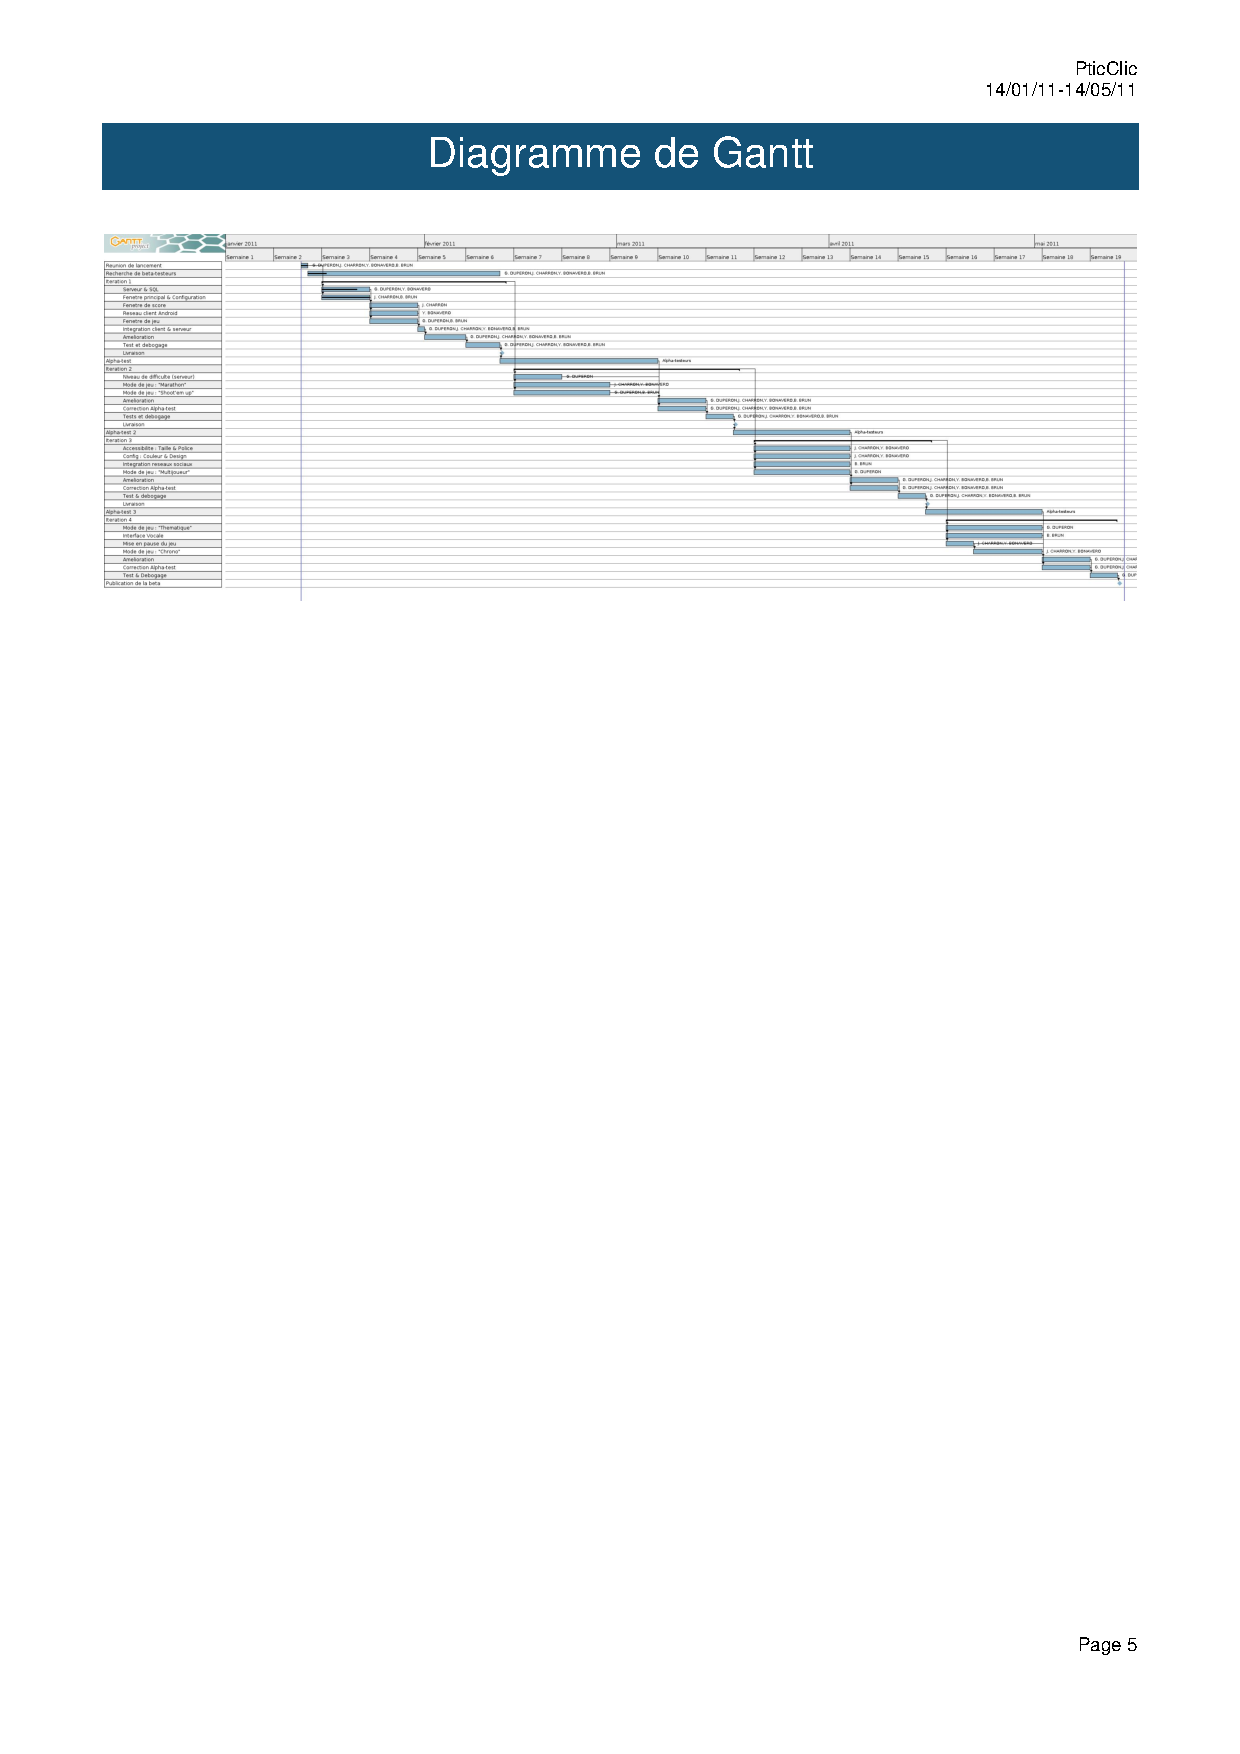
\includegraphics[trim=1.7cm 19cm 1.7cm 4cm,clip,width=20cm]{../feuille-route/gp-pticlic.pdf}
\newpage

\section{Annexe A}


\subsection{14 janvier 2010}


Durée du projet 4 mois (4 itérations de 4 semaines)

Conventions de code : \url{http://java.sun.com/docs/codeconv/html/CodeConventions.doc6.html}

Code (noms de variables, etc.) en anglais, commentaires en français, javadoc en français.

\subsection{26 janvier 2011}
Mettre le serveur (PHP) sur free.fr, pour pouvoir tester facilement

Utilisation d'une classe \verb!Constant!

Écran d'accueil du jeu : Image (splash), puis directement les icônes des modes de jeu + configuration, au lieu d'avoir un écran avec le logo et jouer/config, suivi du choix du mode de jeu.

\section{Annexe B}

%\subsection{Serveur}

****SQL****
2011-m1s2-ter\/code\/serveur\$ ls
02122011-LEXICALNET-JEUXDEMOTS-FR-NOHTML.txt  -- dump de Lafourcade
dump.url -- contient l'URL du dump le plus récent
dump2mysql.sh -- Script pour convertir dump de Lafourcade en sql (pas terminé~? On utilise sqlite, donc on a laissé tombé~?)
dump2sqlite.sh  -- Script pour convertir dump de Lafourcade en sql
parties.json  -- ??
README.sh -- Ce n'est pas un README, c'est un script pour faire l'ensemble de la création de la BD, du téléchargement à la création d'indexes en passant par la création des tables et les insertions.
sql -- Le script sql à proprement parler
php\/db -- fichier binaire sqlite pour le chargement de la bd
php\/db.old -- fichier binaire sqlite pour le chargement de la bd, version précédente (backup)
dossier: select

****SERVEUR****
php\/db.php -- fichier pour ouvrir et fermer ou récupérer l'instance de l'ouverture de la base de données à l'aide d'un singleton. 
		Fichier très court, deux fonctions seulement.
php\/pticlic.php -- contient un grand nombre de fonctions pour le jeu
php\/relations.php -- contient un tableau et les phrases 'relation'
php\/server.php --
php\/showGame.php -- ??



****SITE****
php\/contact.php
php\/createGame.php
php\/download.php
php\/index.php
php\/login.php
php\/showGame.php -- ??
php\/signup.php
php\/ressources/backend.css  -- CSS pour showGame.php
php\/ressources/footer.inc  -- pied de pages du site
php\/ressources/locations.inc  -- petit fichier facilitant la navigation de page en page
php\/ressources/menu.inc  -- menu du site
php\/ressources/pticlic-alpha-v0.1.apk  -- exécutable PtiClic (fichier d'installation de l'application)
php\/ressources/showmsg.inc  -- ?? (pour l'affichage des messages... mais dans quel contexte~? Pourquoi~?)
php\/ressources/simple.css  -- CSS de base du site
php\/ressources/strings.inc -- fichier de configuration des strings (phrases utilisés de manière répétitive dans le site, par exemple, les messages d'erreurs)

\section{Mentions légales}
Android is a trademark of Google Inc. Use of this subject to Google Permissions.

\end{document}
